\documentclass[12pt]{report}

% Pakete
\usepackage{ngerman,a4}
\usepackage[latin1]{inputenc}
\usepackage{makeidx}
\usepackage{exscale,icomma}
\usepackage{amsbsy,amscd,amsfonts,amsmath,amssymb,amstext,amsthm,amsxtra,eqname}
\usepackage[pdftex]{graphicx}
\usepackage[pdftex]{hyperref} \hypersetup{colorlinks,linkcolor=darkblue,filecolor=darkgreen,urlcolor=darkred,citecolor=darkblue}

% Farben
\usepackage{color}
\definecolor{darkred}{rgb}{0.5,0,0}
\definecolor{darkgreen}{rgb}{0,0.5,0}
\definecolor{darkblue}{rgb}{0,0,0.5}

% Protokollierung eines Indexverzeichnisses
\makeindex

% L�ngen festlegen
\setlength{\parindent}{0pt}

% Kurzbefehle: Indexverzeichnis
\newcommand{\wichtig}[1]{\emph{#1}\index{#1}}

% Kurzbefehle: Abstand und Nummerierung
\newcommand{\platz}{\hspace{0.3cm}}
\newcommand{\abstand}{\vspace{0.3cm}}
\newcommand{\seite}{\pagebreak[3]}
\newcommand{\willbuch}{\renewcommand{\labelenumi}{\alph{enumi})}}
\newcommand{\willaberpunkt}{\renewcommand{\labelitemii}{$\bullet$}}

% Kurzbefehle: Mathematik
\newcommand{\nat}{\mathbb{N}}   \newcommand{\natpos}{\mathbb{N}^+}  \newcommand{\ganz}{\mathbb{Z}}
\newcommand{\rat}{\mathbb{Q}}   \newcommand{\ratpos}{\mathbb{Q}^+}
\newcommand{\real}{\mathbb{R}}  \newcommand{\realpos}{\mathbb{R}^+}
\newcommand{\tr}{\; | \;}
\newcommand{\pot}{\mathcal{P}}
\newcommand{\bigO}{\mathcal{O}}
\newcommand{\stime}{\text{\emph{time}}}  \newcommand{\sntime}{\text{\emph{ntime}}}
\newcommand{\btime}{\mathsf{TIME}}       \newcommand{\bntime}{\mathsf{NTIME}}
\newcommand{\bigP}{\mathsf{P}}  \newcommand{\bigNP}{\mathsf{NP}}

\begin{document}

% Titelseite
\title{Grundlagen der theoretischen Informatik}
\author{Institut f�r Informatik \\ Freie Universit�t Berlin \\ Dozent: Dr. Klaus Kriegel \\ \\ Mitschrift: Jan Sebastian Siwy}
\date{Sommersemester 2002}
\maketitle

% Inhaltsverzeichnis
\tableofcontents

% Inhalt
\chapter*{Einleitung} \addcontentsline{toc}{chapter}{Einleitung}
\textbf{Definition:\;} Eine \wichtig{Berechnung} ist ein Prozess, der f�r eine beliebige Eingabe aus einem Eingaberaum in endlich vielen elementaren, deterministischen Schritten eine vorher spezifizierte Ausgabe bestimmt. \abstand

\textbf{Beispiel:}
\begin{itemize}
    \item ganze Zahl $\Rightarrow$ Primzahlzerlegung
    \item Graph mit Kantengewichten $\Rightarrow$ MST (minimal aufspannender Baum)
    \item Polynom �ber $\rat$ $\Rightarrow$ Nullstelle
\end{itemize}
\seite%

\textbf{Themen der Vorlesung:}
\begin{itemize}
    \item Modelle f�r Berechnung
    \item Gemeinsamkeiten (Simulation) und Unterschiede
    \item Berechenbarkeit und Endscheidbarkeit
    \item Church'sche These
    \item Komplexit�t einer Berechnung
    \item P-NP-Problem
    \item Kontextfreie Sprachen
    \item Grammatiken und die Chomsky-Hierarchie
\end{itemize}
\pagebreak

\textbf{Beispiel:}
\begin{enumerate}
    \item Entwurf eines endlichen Automaten zur Steuerung einer Ausgangst�r mit Eingangssperre: \par
    \begin{center}
        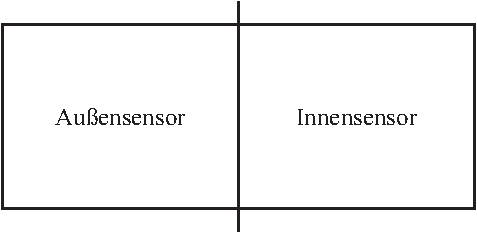
\includegraphics{skript/grafiken/ausgangstuerbild}
    \end{center}
    \begin{tabular}{lccl}
        Eingaben:\; & I & -- & nur Innensensor \\
        & A & -- & nur Au�ensensor \\
        & B & -- & beide \\
        & K & -- & keiner
    \end{tabular}
    \begin{center}
        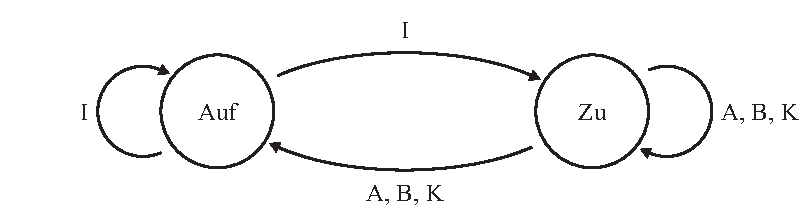
\includegraphics{skript/grafiken/ausgangstuerzustand}
    \end{center}
    \item Postsches Korrespondenzproblem: \\
    Alphabet $\Sigma$ mit den W�rtern $w_1, w_2, \ldots, w_k$ und $v_1, v_2, \ldots, v_k$ \\
    Eingabe: $(w_1, v_2), (w_2, v_2), \ldots (w_k, v_k)$ \\
    Frage: Gibt es eine Indexfolge (mit Wiederholungen) $i_1, i_2, \ldots, i_n$, so dass $w_{i_1} w_{i_2} \ldots w_{i_n} = v_{i_1} v_{i_2} \ldots v_{i_n}$? \\
    Zwei aller m�glichen Eingaben:
    \begin{enumerate}
        \item $\overbrace{(1,101)}^a, \overbrace{(10,00)}^b, \overbrace{(011,11)}^c$ \\
        Indexfolge: $a, c, b, c$ \\
        linke Seite: $1 \; 011 \; 10 \; 011$ \\
        rechte Seite: $101 \; 11 \; 00 \; 11$
        \item $(001,0), (01,011), (01,101), (10,001)$ \\
        k�rzeste L�sung: 66 Paare
    \end{enumerate}
    Dieses Problem ist im Allgemeinen nicht entscheidbar (siehe \ref{entscheidbar})!
\end{enumerate}
\seite

\chapter{Regul�re Sprachen}

%%%%%%%%%%%%%%%%%%%%%%%%%%%%%%%%%%%%%%%%%%%%%%%%%%%%%%%%%%%%%%%%%%%%%%%%%%%%%%%
% Formale Sprachen
%%%%%%%%%%%%%%%%%%%%%%%%%%%%%%%%%%%%%%%%%%%%%%%%%%%%%%%%%%%%%%%%%%%%%%%%%%%%%%%
\section{Formale Sprachen}

%%%%%%%%%%%%%%%%%%%%%%%%%%%%%%%%%%%%%%%%%%%%%%%%%%%%%%%%%%%%%%%%%%%%%%%%%%%%%%%
\subsection{Alphabet}
\textbf{Definition:\;} Ein \emph{endliches Alphabet}\index{Alphabet endlich} ist eine Menge von Symbolen. Alphabete werden h�ufig mit $\Sigma$ oder $\Gamma$ bezeichnet. \par \abstand
\textbf{Beispiel:\; } $\Sigma = \{0, 1\}$, $\Gamma = \{a, b, c, \ldots z\}$

%%%%%%%%%%%%%%%%%%%%%%%%%%%%%%%%%%%%%%%%%%%%%%%%%%%%%%%%%%%%%%%%%%%%%%%%%%%%%%%
\subsection{Wort}
\textbf{Definition:\;} Ein \wichtig{Wort} (String) �ber $\Sigma$ ist eine endliche Folge von Symbolen aus~$\Sigma$, wobei Wiederholungen erlaubt sind. Das \emph{leere Wort}~$\varepsilon$ ($\varepsilon \not\in \Sigma$) besteht aus null Symbolen. Die L�nge des Wortes $|w|$ ist die Anzahl der Symbole in $w$. \par \abstand
\textbf{Beispiel:\;} $w_1 = 01101$, $w_2 = abracadabra$

%%%%%%%%%%%%%%%%%%%%%%%%%%%%%%%%%%%%%%%%%%%%%%%%%%%%%%%%%%%%%%%%%%%%%%%%%%%%%%%
\subsection{Wortmengen}
Um die Menge von W�rtern, die sich aus einem Alphabet bilden lassen, darzustellen, wird folgende Notation vereinbart:
\begin{eqnarray*}
    \Sigma^0 &=& \{ \varepsilon \} \\
    \Sigma^1 &=& \Sigma \\
    \Sigma^{k+1} &=& \{ wa \tr w \in \Sigma^k \wedge a \in \Sigma \} \\
    \Sigma^* &=& \bigcup_{n=0}^\infty \Sigma^n \platz \text{(Menge aller W�rter �ber $\Sigma$)} \\
    \Sigma^+ &=& \bigcup_{n=1}^\infty \Sigma^n \platz \text{(Menge aller W�rter �ber $\Sigma$ ohne das leere Wort)}
\end{eqnarray*}

%%%%%%%%%%%%%%%%%%%%%%%%%%%%%%%%%%%%%%%%%%%%%%%%%%%%%%%%%%%%%%%%%%%%%%%%%%%%%%%
\subsection{Konkatenation}
\textbf{Definition:\;} Die Operation der \wichtig{Konkatenation} in $\Sigma^*$ verbindet zwei W�rter. Das Wort $w$ konkateniert mit dem Wort $w'$ ist $ww'$. $\Sigma^*$ mit der Konkatenation ist ein Monoid. \par \abstand
F�r die Konkatenation gleicher W�rtern wird folgede Nolation vereinbart:
\begin{eqnarray*}
    w^0 &=& \varepsilon \\
    w^1 &=& w \\
    w^{k+1} &=& ww^k \\ \\
    |w^k| &=& k \cdot |w|
\end{eqnarray*}
\textbf{Beispiel:\;} $1011$ konkateniert mit $011$ ist $1011011$. \par \abstand

%%%%%%%%%%%%%%%%%%%%%%%%%%%%%%%%%%%%%%%%%%%%%%%%%%%%%%%%%%%%%%%%%%%%%%%%%%%%%%%
\subsection{Formale Sprachen}
\textbf{Definition:\;} Eine Untermenge $L \subseteq \Sigma^*$ wird \emph{formale Sprache}\index{Sprache, formal} �ber $\Sigma$ genannt. \par \abstand
\textbf{Definition:\;} Die folgenden Operationen auf Sprachen nennt man \wichtig{regul�r}:
\begin{enumerate}
    \item Vereinigung: $A \cup B = \{w \tr w \in A \vee w \in B\}$
    \item Konkatenation: $A \circ B = \{ww' \tr w \in A \wedge w' \in B\}$
    \item Stern: $A^* = \{w_1 w_2 \ldots w_k \tr k \in \nat, w_i \in A\}$
\end{enumerate}
\seite
\textbf{Beispiele:}
\begin{eqnarray*}
    A &=& \{\text{good}, \text{bad}\} \\
    B &=& \{\text{girl}, \text{boy}\} \\
    A \cup B &=& \{\text{good}, \text{bad}, \text{girl}, \text{boy}\} \\
    A \circ B &=& \{\text{goodgirl}, \text{badgirl}, \text{goodboy}, \text{badboy}\} \\
    A^* &=& \{\varepsilon, \text{good}, \text{bad}, \text{goodgood}, \text{goodbad}, \text{badgood}, \text{badbad}, \text{goodgoodgood}, \ldots \}
\end{eqnarray*}
\pagebreak


%%%%%%%%%%%%%%%%%%%%%%%%%%%%%%%%%%%%%%%%%%%%%%%%%%%%%%%%%%%%%%%%%%%%%%%%%%%%%%%
% Endliche Automaten
%%%%%%%%%%%%%%%%%%%%%%%%%%%%%%%%%%%%%%%%%%%%%%%%%%%%%%%%%%%%%%%%%%%%%%%%%%%%%%%
\section{Endliche Automaten}

%%%%%%%%%%%%%%%%%%%%%%%%%%%%%%%%%%%%%%%%%%%%%%%%%%%%%%%%%%%%%%%%%%%%%%%%%%%%%%%
\subsection{Deterministische Automaten}
\textbf{Definition:\;} Ein \wichtig{deterministischer endlicher Automat} (deterministic finite automaton, kurz \wichtig{DFA}) $M$ ist ein 5-Tupel:
$$ M = (Q, \Sigma, \delta, q_0, F) $$
\begin{itemize}
    \item $Q$: endliche Menge von Zust�nden
    \item $\Sigma$: Eingabealphabet
    \item $\delta$: Zustands�berf�hrungsfunktion ($Q \times \Sigma \rightarrow Q$)
    \item $q_0 \in Q$: Anfangszustand
    \item $F$: Menge der akzeptierenden Zust�nde
\end{itemize}
Ein DFA kann als gerichteter Graph dargestellt werden: \label{DFA1}
\begin{center}
    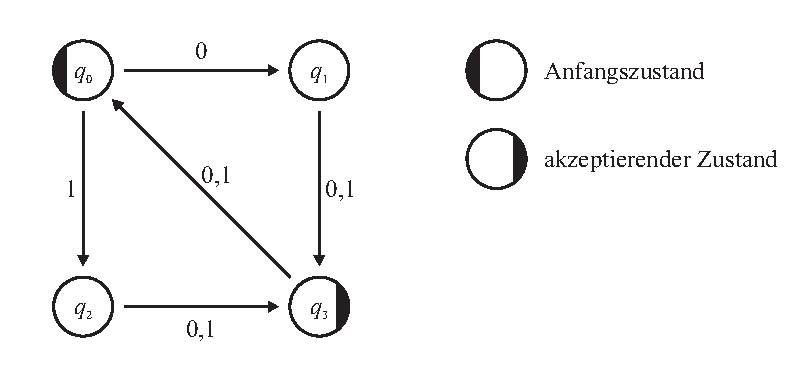
\includegraphics{skript/grafiken/dfa1}
\end{center}
F�r jedes $q \in Q$ und $a \in \Sigma$ gibt es genau eine Kante von $q$ mit dem Wert $a$.
\pagebreak

%%%%%%%%%%%%%%%%%%%%%%%%%%%%%%%%%%%%%%%%%%%%%%%%%%%%%%%%%%%%%%%%%%%%%%%%%%%%%%%
\subsection{Akzeptierte Sprachen von DFAs}
Um Berechnungen durchf�hren zu k�nnen, wird die Zustand�berf�hrungsfunktion $\delta$ induktiv erweitert, so dass sie W�rter verarbeiten kann.
\begin{eqnarray*}
    \hat{\delta} & : & Q \times \Sigma^* \rightarrow Q \\
    \hat{\delta}(q,\varepsilon) &=& q \\
    \hat{\delta}(q,aw) &=& \hat{\delta}(\delta(q,a),w)
\end{eqnarray*}
\textbf{Definition:\;} Ein Wort $w \in \Sigma^*$ wird genau dann akzeptiert, wenn $\hat{\delta}(q_0,w) \in F$. \par \abstand
\textbf{Definition:\;} Die Menge aller akzeptierten W�rter bildet die \wichtig{akzeptierte Sprache} des Automaten:
$$ L(M) = \{w \in \Sigma^* \tr \hat{\delta}(q,w) \in F \} $$
\textbf{Beispiel:\;} Die akzeptierte Sprache des Automanten im Abschnitt~\ref{DFA1} lautet:
$$ L(M) = \{ w \tr w \in \{0,1\}^*, |w|=3k+2, k \in \nat \} $$

%%%%%%%%%%%%%%%%%%%%%%%%%%%%%%%%%%%%%%%%%%%%%%%%%%%%%%%%%%%%%%%%%%%%%%%%%%%%%%%
\subsection{"`Sackgassen"'-Prinzip}
Entwurf eines Automaten, der alle alterierenden 01-Folgen akzeptiert. \par \abstand
\begin{center}
    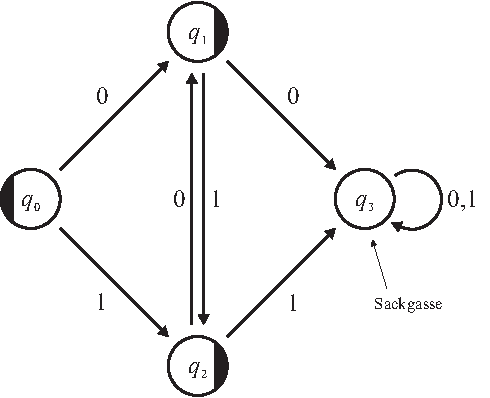
\includegraphics{skript/grafiken/dfaalterier}
\end{center}
Das "`Sackgassen"'-Prinzips beruht darauf, dass ein Zustand existiert, bei dem die Zustands�bergangsfunktion f�r alle Eingaben wieder denselben Zustand liefert. Dies ist n�tzlich, wenn ab einer bestimmten Stelle im Wort bekannt ist, dass dieses Wort mit Sicherheit akzeptiert bzw. nicht akzeptiert werden soll.

%%%%%%%%%%%%%%%%%%%%%%%%%%%%%%%%%%%%%%%%%%%%%%%%%%%%%%%%%%%%%%%%%%%%%%%%%%%%%%%
\subsection{�quivalenz}
\textbf{Definition:\;} Zwei Automaten $M$ und $M'$ sind \emph{�quivalent}\index{�quivalenz} wenn deren Sprachen $L(M)$ und $L(M')$ gleich sind. \par \abstand
\textbf{Beispiel:\;} Der folgende Automat ist �quivalent zum Automaten im Abschnitt~\ref{DFA1}, da er der gleiche Sprache akzeptiert.
\begin{center}
    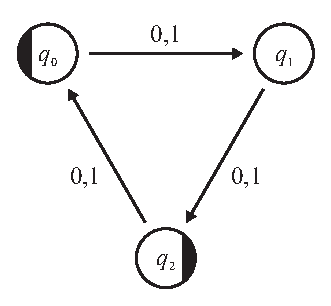
\includegraphics{skript/grafiken/dfa2}
\end{center}

%%%%%%%%%%%%%%%%%%%%%%%%%%%%%%%%%%%%%%%%%%%%%%%%%%%%%%%%%%%%%%%%%%%%%%%%%%%%%%%
\subsection{Vereinigung von DFA-Sprachen}\label{dfaverein}
\textbf{Satz:\;} Sind $A$ und $B$ DFA-Sprachen, dann ist auch $A \cup B$ auch DFA-Sprache. \par \abstand

\textbf{Beweis:\;} Beide Automaten sollen parallel arbeiten. Es sollen alle W�rter akzeptiert werden, welche der erste \emph{oder} der zweite Automat akzeptiert. Dazu bildet man das kartisiches Produkt der Zustandsmengen von $M_1$ und $M_2$.
\begin{eqnarray*}
    \delta &:& ((Q_{M_1}, Q_{M_2}), \Sigma) \rightarrow (Q_{M_1}, Q_{M_2}) \\
    \delta((q_{M_1}, q_{M_2}), a) &=& (\delta_{M_1}(q_{M_1},a), \delta_{M_2}(q_{M_2}, a) ) \\
    F &=& \{ (q_{M_1}, q_{M_2}) \tr q_{M_1} \in F_{M_1} \; \vee \; q_{M_2} \in F_{M_2} \} \\
    L(M) &=& A \cup B
\end{eqnarray*}
\pagebreak

\textbf{Beispiel:\;} Es sind gegeben die beiden folgenden Automaten $M_1$ und $M_2$ mit den Sprachen $A$ und $B$.
\begin{eqnarray*}
    A = L(M_1) &=& \{ (01)^k \tr k \in \nat \} = (01)^* \\
    B = L(M_2) &=& \{ (10)^k \tr k \in \nat \} = (10)^*
\end{eqnarray*}
\begin{center}
    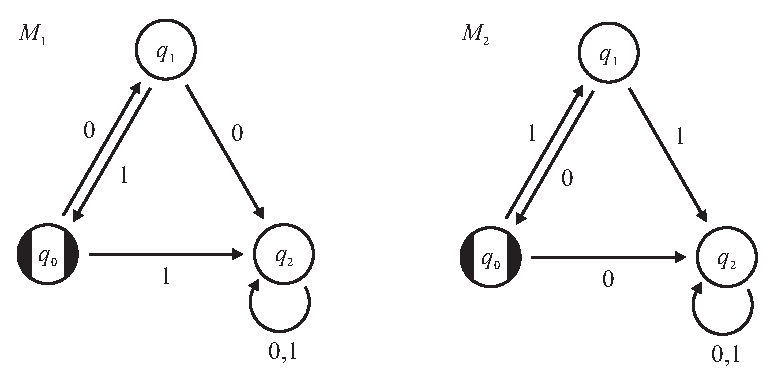
\includegraphics{skript/grafiken/dfavereinigung1}\label{Vereinigung}
\end{center}
Die Vereinigung der beiden Sprachen $A$ und $B$ lautet:
$$A \cup B = \{ w \tr w \in (01)^* \vee w \in (10)^* \}$$
\begin{center}
    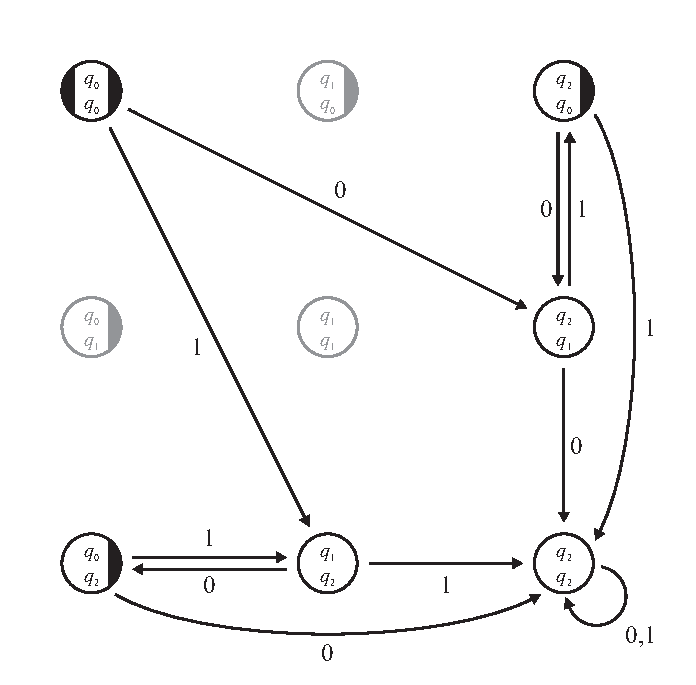
\includegraphics{skript/grafiken/dfavereinigung2}
\end{center}

%%%%%%%%%%%%%%%%%%%%%%%%%%%%%%%%%%%%%%%%%%%%%%%%%%%%%%%%%%%%%%%%%%%%%%%%%%%%%%%
\subsection{Nichtdeterministische Automaten}

\textbf{Definition:\;} Ein \wichtig{nichtdeterministischer endlicher Automat} (nondeterministic finite automaton, kurz \wichtig{NFA}) $M$ ist ein 5-Tupel:
$$ M = (Q, \Sigma, \delta, q_0, F) $$
\begin{itemize}
    \item $Q$: Menge von Zust�nden
    \item $\Sigma$: endliches Eingabealphabet
    \item $\delta$: Zustands�berf�hrungsfunktion ($Q \times \Sigma \rightarrow \pot(Q)$)
    \item $q_0$: Anfangszustand
    \item $F$: Menge der akzeptierenden Zust�nde
\end{itemize}
\seite

\textbf{Beispiel:\;} Dieser NFA akzeptiert alle W�rter, deren vorletztes Symbol $1$ ist.
\begin{center}
    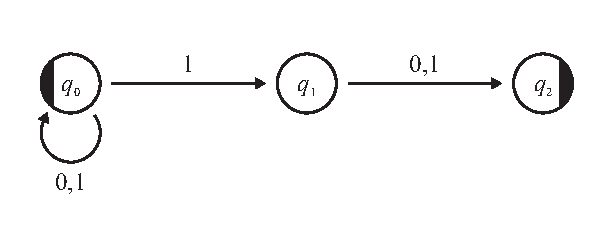
\includegraphics{skript/grafiken/nfavorletzte1} \label{NFA1}
\end{center}

%%%%%%%%%%%%%%%%%%%%%%%%%%%%%%%%%%%%%%%%%%%%%%%%%%%%%%%%%%%%%%%%%%%%%%%%%%%%%%%
\subsection{Akzeptierte Sprachen von NFAs}
Um eine Berechnungen durchf�hren zu k�nnen, wird die Zustand�berf�hrungsfunktion $\delta$ erweitert, so dass sie W�rter verarbeiten kann.
\begin{eqnarray*}
    \hat{\delta} &:& \pot(Q) \times \Sigma^* \rightarrow \pot(Q) \\
    \hat{\delta}(S, \varepsilon) &=& S \\
    \hat{\delta}(S, aw) &=& \hat{\delta} \left( \bigcup_{q \in S} \delta(q, a), w \right)
\end{eqnarray*}
\textbf{Definition:\;} Ein Wort $w \in \Sigma^*$ wird von $M$ genau dann akzeptiert, wenn es mindestens einen Berechnungszweig f�r $w$ gibt, der von $q_0$ zu einem $q \in F$ f�hrt.
$$ \hat{\delta}\left( \{q_0\}, w \right) \cap F \neq \emptyset $$
\pagebreak

%%%%%%%%%%%%%%%%%%%%%%%%%%%%%%%%%%%%%%%%%%%%%%%%%%%%%%%%%%%%%%%%%%%%%%%%%%%%%%%
\subsection{Simulation eines NFA durch einen DFA}
\textbf{Satz:\;} Jeder NFA kann durch einen �quivalenten DFA \emph{simuliert}\index{Simulation eines NFA} werden. \par \abstand

\textbf{Beweis:\;} Die Zust�nde des DFA $M'$ werden repr�sentiert durch alle Teilmengen der Zustandsmenge von des NFA $M$.
\begin{eqnarray*}
    M = (Q, \Sigma, \delta, q_0, F) & \Rightarrow & M' = (\pot(Q), \Sigma, \delta', \{q_0\}, F') \\ \\
    & & \delta'(S, a) = \bigcup_{q \in S} \delta(q, a) \\ \\
    & & F' = \{S \in \pot(Q) \tr S \cap F \neq \emptyset \} \\ \\
    L(M) &=& L(M')
\end{eqnarray*}
\seite

\textbf{Beispiel:\;} Der folgende DFA ist �quivalent zum NFA im Abschnitt~\ref{NFA1}.
\begin{center}
    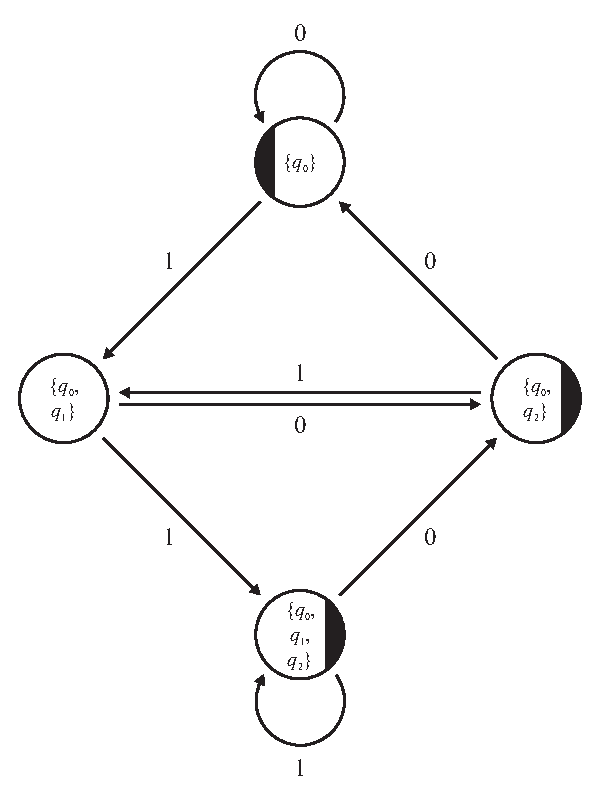
\includegraphics{skript/grafiken/nfavorletzte2} \label{NFA2}
\end{center}

%%%%%%%%%%%%%%%%%%%%%%%%%%%%%%%%%%%%%%%%%%%%%%%%%%%%%%%%%%%%%%%%%%%%%%%%%%%%%%%
\subsection{$\varepsilon$-�berg�nge}
\textbf{Definition:\;} $M$ ist ein NFA mit \emph{$\varepsilon$-�berg�ngen}\index{$\varepsilon$-�berg�nge}, wenn die Zustands�bergangsfunktion $\delta$ auch "`spontane"' Zustand�berg�nge (also Zustand�berg�nge ohne Verarbeitung eines Symbols $a$ aus $\Sigma$) zul�sst:
$$\delta \; : \; Q \times (\Sigma \cup \{ \varepsilon \})~\Rightarrow~\pot(Q)$$
$M$ akzeptiert eine Eingabe $w \in \Sigma^*$, wenn es einen Zweig der Berechnung gibt, der von $q_0$ zu einem akzeptierenden Zustand f�hrt, dessen konkatenierte Berechnung~$w$ ist. \par \abstand
\textbf{Anwendung:\;} Konkatenation der Sprachen von $M_1$ und $M_2$ aus Abschnitt \ref{Vereinigung}.
\begin{center}
    \includegraphics{skript/grafiken/nfaepsilonKonkat1}
\end{center}
\textbf{Satz:\;} Jeder NFA $M$ mit $\varepsilon$-�berg�ngen kann durch einen NFA $M'$ ohne $\varepsilon$-�berg�nge simuliert werden. $Q$, $\Sigma$, $q_0$ und $F$ bleiben dabei gleich, jedoch muss die Zustands�bergangsfunktion angepasst werden:
$$ \delta'(q, a) = \bigcup_{i, j \in \nat} \hat{\delta}(q, \varepsilon^i a \varepsilon^j) \platz \platz \platz \text{(f�r $i, j \in \nat$)} $$
Ausnahme: Falls der Automat mit $\varepsilon$-�berg�ngen das leere Wort $\varepsilon$ akzeptiert, dann muss die Menge der akzeptierenden Zust�nde um den Startzustand $q_0$ erweitert werden.
$$ \delta (q_0, \varepsilon) \cap F \neq \emptyset \platz \Rightarrow \platz q_0 \in F' $$
\pagebreak

\textbf{Beispiel:\;} Aufl�sung der $\varepsilon$-�berg�nge
\begin{center}
    \includegraphics{skript/grafiken/nfaepsilonKonkat2}
\end{center}

\subsection{Konkatenation und Stern von DFA-Sprachen}\label{dfakonkat}
\textbf{Satz:\;} DFA-Sprachen sind abgeschlossen gegen�ber der Konkatenation und dem~Stern. \par \abstand
\textbf{Beweis:\;} $M_1$ ist DFA f�r $A$ und $M_2$ ist DFA f�r $B$.
\begin{itemize}
    \item Schritt 1: Konstruktionen von NFAs mit $\varepsilon$-�berg�ngen f�r $A \circ B$ und $A^*$.
    \begin{itemize}
        \item $M^{\circ}$ f�r $A \circ B$
        \begin{itemize}
            \item disjukte Vereinigung der Zustandsmengen von $M_1$ und $M_2$
            \item f�r jedes $q \in F_{M_1}$ ein $\varepsilon$-�bergang nach $q_{0,M_2}$
            \item $F_{M^{\circ}} = F_{M_1}$
            \item $q_{0, M^{\circ}} = q_{0, M_1}$
        \end{itemize}
        \begin{center}
            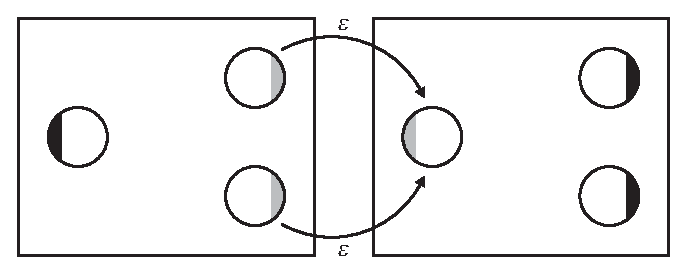
\includegraphics{skript/grafiken/dfakonkat}
        \end{center}
        \seite
        \item $M^*$ f�r $A^*$
        \begin{itemize}
            \item Zustandsmenge von $M_1$ und neuer Startzustand $q_{-1}$
            \item $\varepsilon$-�bergang von $q_{-1}$ nach $q_0$
            \item f�r jedes $q \in F_{M_1}$ ein $\varepsilon$-�bergang nach $q_0$
        \end{itemize}
        \begin{center}
            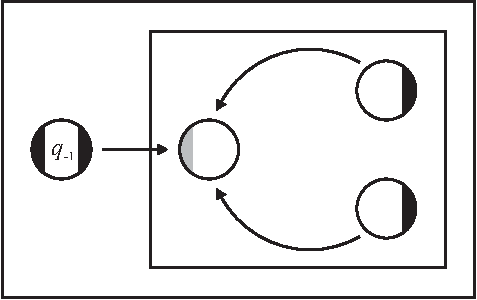
\includegraphics{skript/grafiken/dfastern}
        \end{center}
    \end{itemize}
    \item Schritt 2: Umwandlung der NFAs mit $\varepsilon$-�berg�ngen in �quivalente NFAs ohne~$\varepsilon$-�berg�nge
    \item Schritt 3: Umwandlung der NFAs ohne $\varepsilon$-�berg�nge in �quivalente DFAs
\end{itemize}
\pagebreak

%%%%%%%%%%%%%%%%%%%%%%%%%%%%%%%%%%%%%%%%%%%%%%%%%%%%%%%%%%%%%%%%%%%%%%%%%%%%%%%
% Minimierung endlicher Automanten
%%%%%%%%%%%%%%%%%%%%%%%%%%%%%%%%%%%%%%%%%%%%%%%%%%%%%%%%%%%%%%%%%%%%%%%%%%%%%%%
\section{Minimierung endlicher Automanten}

%%%%%%%%%%%%%%%%%%%%%%%%%%%%%%%%%%%%%%%%%%%%%%%%%%%%%%%%%%%%%%%%%%%%%%%%%%%%%%%
\subsection{Unerreichbare und �quivalenze Zust�nde}
\textbf{Ziel:\;} $L$ sei DFA-Sprache. Man konstruiert einen DFA $M$, so dass $L(M) = L$ und die Anzahl der Zust�nde $|Q_M|$ minimal ist. \par \abstand
\textbf{L�sung:}
\begin{enumerate}
    \item Eleminierung unerreichbarer Zust�nde
    \item Verschmelzung �quivalenter Zust�nde
\end{enumerate} \abstand \abstand

\textbf{Definition:\;} $q \in Q$ ist \wichtig{unerreichbar}, wenn es keine Eingabe $w \in \Sigma^*$ gibt, die zu diesem Zustand $q$ f�hrt.
$$ \forall w \in \Sigma^* \platz q \neq \hat{\delta}(q_0, w) $$
\textbf{Satz:\;} Die Menge der unerreichbaren Zust�nde eines DFAs kann in $O(|Q| \cdot |\Sigma|)$ Zeit bestimmt werden. F�r den durch die erreichbaren Zust�nde induzierten Automaten $M'$ gilt $L(M') = L(M)$. \par \abstand
\textbf{Beweis:\;} DFS oder BFS im Graphen des Automaten  mit Start in $q_0$ liefert alle erreichbaren Zust�nde, die restlichen sind nicht erreichbar. Die zweite Behauptung ergibt sich aus der Definition von $\hat{\delta}$. \par \abstand \abstand

\textbf{Definition:\;} $M$ ist ein DFA. Zwei Zust�nde $q, q' \in Q$ hei�en \emph{�quivalent}\index{�quivalenze Zust�nde}, wenn f�r alle $w \in \Sigma^*$ gilt
$$ \hat{\delta}(q, w) \in F \platz \Leftrightarrow \platz \hat{\delta}(q', w) \in F $$
Wir schreiben dann $q \equiv q'$. $\equiv$ ist eine �quivalenzrelation.
\pagebreak

%%%%%%%%%%%%%%%%%%%%%%%%%%%%%%%%%%%%%%%%%%%%%%%%%%%%%%%%%%%%%%%%%%%%%%%%%%%%%%%
\subsection{�quivalenzklassenautomat}
\textbf{Definition:\;} Der \wichtig{�quivalenzklassenautomat} $M'$ von $M$ hat die folgende Gestalt:
\begin{itemize}
    \item $Q' = Q_{/ \equiv}$ (Menge der �quivalenzklassen)
    \item $\Sigma' = \Sigma$
    \item $q_0' = [q_0]_{\equiv}$
    \item $F' = \{ [q]_{\equiv} \tr q \in F \}$
    \item $\delta'([q]_{\equiv}, a) = [\delta(q, a)]_{\equiv} \in Q'$
\end{itemize}

\textbf{Beweise:}
\begin{enumerate}
    \item $F'$ ist wohldefiniert. \par
    Zu zeigen ist: Aus $q \equiv q'$ folgt, dass $q \in F \Leftrightarrow q' \in F$. \par
    Dazu muss man $q \equiv q'$ mit dem Wort $w = \varepsilon$ in die Definition von $\equiv$ einsetzen.
    \begin{eqnarray*}
        \hat{\delta}(q, \varepsilon) \in F &\Leftrightarrow& \hat{\delta}(q', \varepsilon) \in F \\
        q \in F &\Leftrightarrow& q' \in F
    \end{eqnarray*}
    \item $\delta'$ ist wohldefiniert. \par
    Zu zeigen ist: Aus $q \equiv q'$ folgt, dass $\forall a \in \Sigma \platz \delta'([q]_{\equiv}, a) = \delta'([q']_{\equiv}, a)$ \par
    Aus $q \equiv q'$ folgt, dass $\forall w \in \Sigma^* \platz \hat{\delta}(q, w) \in F \Leftrightarrow \hat{\delta}(q', w) \in F$. \par
    Insbesondere gilt f�r jedes $w = aw'$: $\hat{\delta}(q, aw') \in F \Leftrightarrow \hat{\delta}(q', aw') \in F$. \par
    Laut Definition von $\hat{\delta}$ ist $\hat{\delta}(q, aw') = \hat{\delta}(\delta(q, a), w')$. \par
    Das bedeutet, dass $\hat{\delta}(\delta(q, a), w) \in F \Leftrightarrow \hat{\delta}(\delta(q', a), w) \in F$. \par
    Daraus folgt: $\delta(q, a) \equiv \delta(q', a)$, also $\delta'([q]_{\equiv}, a) = \delta'([q']_{\equiv}, a)$.
    \item $L(M) = L(M')$. \par
    Aus $w {\in \atop \notin} L(M)$ folgt, dass die Zustandsfolge $q_0, q_1, \ldots q_n$ mit $q_n {\in \atop \notin} F$ endet. Die entsprechende Zustandfolge $[q_0]_{\equiv}, [q_1]_{\equiv}, \ldots [q_n]_{\equiv}$ f�r den �quivalenzautomaten endet folglich mit $[q_n]_{\equiv} {\in \atop \notin} F'$ folgt.
\end{enumerate}
\pagebreak

\textbf{Konstruktion eines �quivalenzklassenautomaten:}
$$ q \equiv q' \platz \Leftrightarrow \platz \left( \forall w \in \Sigma^* \platz \hat{\delta}(q, w) \in F \Leftrightarrow \hat{\delta}(q', w) \in F \right) $$
Algorithmische Bestimmung von $\equiv$ �ber $\not\equiv$:
\begin{eqnarray*}
    q \not\equiv q' &\Leftrightarrow& \left( \exists w \in \Sigma^* \platz \hat{\delta}(q, w) \in F \wedge \hat{\delta}(q', w) \notin F \right) \text{ oder} \\
                    &               & \left( \exists w \in \Sigma^* \platz \hat{\delta}(q, w) \notin F \wedge \hat{\delta}(q', w) \in F \right)
\end{eqnarray*}

Beobachtung:
\begin{enumerate}
    \item Ist $w = aw'$ Zeuge f�r $q \not\equiv q'$, dann ist $w'$ Zeuge f�r $\delta(q, a) \not\equiv \delta(q', a)$
    \begin{center}
        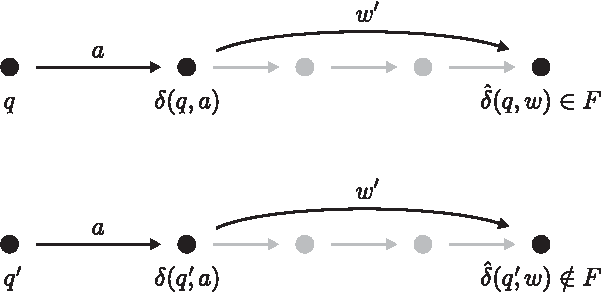
\includegraphics{skript/grafiken/aequivzeugen}
    \end{center}
    \item Ist $w''$ der k�rzeste Zeuge f�r $\delta(q, a) \not\equiv \delta(q', a)$, dann ist $aw''$ ein k�rzester Zeuge f�r $q \not\equiv q'$, der mit $a$ beginnt.
\end{enumerate}

Algorithmus f�r $\not\equiv$:\; Man beginnt mit dem Zeugen $w$ der L�nge $0$ (d.h. $w~=~\varepsilon$). Dann testet man alle Nicht�quivalenzen durch schrittweise Erh�hung der Zeugenl�nge. Wenn nach einer Erh�hung keine \emph{neuen} Nicht�quivalenzen auftreten, stoppt das Verfahren. \par \abstand
\pagebreak

%%%%%%%%%%%%%%%%%%%%%%%%%%%%%%%%%%%%%%%%%%%%%%%%%%%%%%%%%%%%%%%%%%%%%%%%%%%%%%%
\subsection{Nerode-Relation}
\textbf{Definition:\;} F�r $L \subseteq \Sigma^*$ ist $R_L$ in $\Sigma^*$ die \wichtig{Nerode-Relation} (f�r alle $x, y \in \Sigma^*$):
$$ x \; R_L \; y \platz \Leftrightarrow \platz ( \forall w \in \Sigma^* \platz xw \in L \platz \Leftrightarrow \platz yw \in L ) $$
\vspace{0.2cm}

\textbf{Satz:\;} Die Menge der �quivalenzklassen $\Sigma^*_{/ R_L}$ ist genau dann endlich, wenn $L$ eine DFA-Sprache ist. \par \abstand
\textbf{Beweis ($\Rightarrow$):\;} Konstruktion eines DFAs f�r $L$, mit einem Zustand f�r jede �quivalenzklasse~$[x]_{R_L}$ von $R_L$.
\begin{itemize}
    \item $q_0 = [\varepsilon]_{R_L}$
    \item $\delta([x]_{R_L}, a) = [xa]_{R_L}$
    \item $[x]_{R_L} \in F \Leftrightarrow x \in L$
    \item $L(M) = L$
\end{itemize}
Das hei�t, man kann einen DFA konstruieren, sofern die Anzahl der �quivalenzklassen der Nerode-Relation $R_L$ endlich ist. \par \abstand
\textbf{Beweis ($\Leftarrow$):\;} Man w�hle $x, y \in \Sigma^*$ beliebig.
\begin{itemize}
    \item Wenn $\hat{\delta}(q_0, x) = \hat{\delta}(q_0, y)$, dann $ x \; R_L \; y $, somit $[x]_{R_L} = [y]_{R_L}$.
    \item Wenn $\neg (x \; R_L \; y)$, somit $[x]_{R_L} \neq [y]_{R_L}$, dann $\hat{\delta}(q_0, x) \neq \hat{\delta}(q_0, y)$.
\end{itemize}
Daraus folgt, dass es maximal so viele �quivalenzklassen in der Nerode-Relation geben kann wie Zust�nde in einem beliebigen DFA. Damit ist die Anzahl der �quivalenzklassen endlich.
$$ \left| \Sigma^*_{/ R_L} \right| \leq |Q| $$
\vspace{0.2cm}

\textbf{Satz:\;} Die Anzahl der Zust�nde von $M_{\equiv}$ entspricht maximal der Anzahl der �quivalenzklassen von~$R_L$. \par \abstand
\textbf{Beweis:\;} Man w�hle $x, y \in \Sigma^*$ beliebig.
\begin{itemize}
    \item Wenn $x \; R_L\;  y$, dann $\hat{\delta}(q_0, x) \equiv \hat{\delta}(q_0, y)$
    \item Wenn $\hat{\delta}(q_0, x) \not\equiv \hat{\delta}(q_0, y)$, dann $\neg (x \; R_L \; y)$
\end{itemize}
Daraus folgt, dass es maximal so viele Zust�nde im �quivalenzklassenautomaten gibt wie �quivalenzklassen in der Nerode-Relation.
$$ \left| Q_{/ \equiv} \right| \leq \left| \Sigma^*_{/ R_L} \right| $$
\pagebreak

\textbf{Satz:\;} Die �quivalenzklassenautomat $M_{\equiv}$ von $M$ ist ein Minimalautomat f�r~$L(M)$. \par \abstand
\textbf{Beweis:\;} Sei $M''$ ein Minimalautomat f�r $L(M)$, dann folgt daraus:
$$ \left| Q_{/ \equiv} \right|  \leq \left| \Sigma^*_{/ R_L} \right| \leq |Q''| $$
Aber alle $\leq$ sind $=$, sonst w�re $Q''$ nicht minimal. Daraus folgt
$$\left| Q_{/ \equiv} \right| = \left| Q'' \right|$$
und $M_{\equiv}$ ist Minimalautomat. \par \vspace{0.7cm}

\textbf{Beispiel:\;} �berpr�fung mit Hilfe der Nerode-Relation, ob eine Sprache $L$ DFA-Sprache ist.
\begin{itemize}
    \item $L = \{ w \in \{ 0,1 \}^* \tr \text{$w$ beginnt mit $01$} \}$ \par
    �quivalenzklassen von $R_L$
    \begin{itemize}
        \item $[\varepsilon]_{R_L} = \{ \varepsilon \}$
        \item $[0]_{R_L} = \{ 0 \}$
        \item $[1]_{L_R} = \{ 1, 00 \} \circ \Sigma^*$
        \item $[01]_{R_L} = \{ 01 \} \circ \Sigma^*$
    \end{itemize}
    Alle �quivalenzklassen von $R_L$ ergeben wieder $L$:
    $$ L = [\varepsilon]_{R_L} \cup [0]_{R_L} \cup [1]_{R_L} \cup [01]_{R_L} $$
    Da die Anzahl der �quivalenzklassen von $R_L$ endlich ist, ist $L$ DFA-Sprache.
    \item $L = \{ 0^n 1^n \tr n \in \nat \}$ \par
    Die Anzahl der �quivalenzklassen ist unendlich, da $\neg (0^i \; R_L \; 0^j)$ f�r $i \neq j$. \par
    Begr�ndung: F�r $w = 1^i$ ist $0^i \; 1^i \in L$, aber $0^j \; 1^i \notin L$. \par
    Damit ist $L$ keine DFA-Sprache.
\end{itemize}
\pagebreak

%%%%%%%%%%%%%%%%%%%%%%%%%%%%%%%%%%%%%%%%%%%%%%%%%%%%%%%%%%%%%%%%%%%%%%%%%%%%%%%
% Regul�re Sprachen und regul�re Ausdr�cke
%%%%%%%%%%%%%%%%%%%%%%%%%%%%%%%%%%%%%%%%%%%%%%%%%%%%%%%%%%%%%%%%%%%%%%%%%%%%%%%
\section{Regul�re Sprachen und regul�re Ausdr�cke}

%%%%%%%%%%%%%%%%%%%%%%%%%%%%%%%%%%%%%%%%%%%%%%%%%%%%%%%%%%%%%%%%%%%%%%%%%%%%%%%
\subsection{Einf�hrung}
\textbf{Definition:\;} \emph{Regul�re Sprachen}\index{regul�re Sprachen} �ber $\Sigma$ sind induktiv definiert:
\begin{enumerate}
    \item $L = \emptyset$ und $L = \{ a \}$ f�r $a \in \Sigma$ sind regul�r.
    \item Sind $L_1$ und $L_2$ regul�r, dann ist auch $L_1 \cup L_2$ regul�r.
    \item Sind $L_1$ und $L_2$ regul�r, dann ist auch $L_1 \circ L_2$ regul�r.
    \item Ist $L_1$ regul�r, dann ist auch $L^*_1$ regul�r.
\end{enumerate}
Eine vollst�ndige Beschreibung einer regul�ren Sprache durch 1. - 4. nennt man einen \emph{regul�ren Ausdruck}\index{regul�re Ausdr�cke}. \par \abstand

\textbf{Beispiele:}
\begin{itemize}
    \item $L = \{ w \in \{ 0,1 \}^* \tr \text{$w$ beginnt mit 0} \} = 0(\{0\} \cup \{1\})^* = 0 \{0,1\}^* = 0 \Sigma^*$
    \item $L = \{ \varepsilon \} = \emptyset^*$
    \item $L = \{ w \in \{0,1\}^* \tr \text{$w$ hat 3 aufeinander folgende 1} \} = \Sigma^* 111 \Sigma^*$
    \item $L = \{ w \in \{0,1\}^* \tr \text{$w$ enth�lt \emph{nicht} 010} \}$
    \begin{itemize}
        \item Fall 1: 01 tritt nicht auf in $w$: $1^*0^*$
        \item Fall 2: 01 tritt (endlich oft) auf, muss mit 1 weitergehen, au�er beim letzten 01, da dort auch $\varepsilon$ m�glich ist.
    \end{itemize}
    $L = 1^*0^* \cup 1^*0^* (0111^*0^*)^*01(11^*0^* \cup \emptyset^*)$
\end{itemize}
\pagebreak

%%%%%%%%%%%%%%%%%%%%%%%%%%%%%%%%%%%%%%%%%%%%%%%%%%%%%%%%%%%%%%%%%%%%%%%%%%%%%%%
\subsection{Zusammenhang zu DFA-Sprachen}

\textbf{Satz:\;} $L$ ist genau dann eine regul�re Sprache, wenn $L$ DFA-Sprache ist. \par \abstand

\textbf{Beweis ($\Rightarrow$):\;} Man konstruiert einen DFA.
\begin{itemize}
    \item $L = \emptyset$ oder $L = \{ a \}$
    \begin{center}
        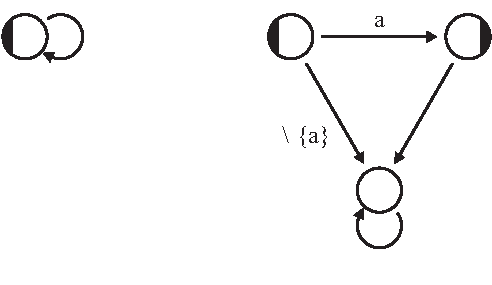
\includegraphics{skript/grafiken/regausdruck}
    \end{center}
    \item $L$ ist Vereinigung, Konkatenation oder Stern. \par \abstand
    $\left. \begin{array}{l@{\platz \rightarrow \platz}l}
    L = L_1 \cup L_2 & L(M) = L(M_1) \cup L(M_2) \\
    L = L_1 \circ L_2 & L(M) = L(M_1) \circ L(M_2) \\
    L = L_1^* & L(M) = L(M^*)
    \end{array} \right\} \text{ (siehe \ref{dfaverein} und \ref{dfakonkat})}$
\end{itemize} \abstand
\textbf{Beweis ($\Leftarrow$):\;} Sei $L$ sei eine DFA-Sprache mit $Q = \{ 1, \ldots n \}$ und dem Anfangszustand $1$. Man konstruiert einen regul�ren Ausdrucks f�r $L$ mit dynamischem Programmieren ($1 \leq i, j \leq n$ und $k \geq 0$):
$$R^k_{i, j} = \{ w \in \Sigma^* \tr \hat{\delta}(i, w) = j \text{ und alle Zwischenzust�nde $\leq k$} \}$$
$R^k_{i, j}$ wird schrittweise aufgebaut $k = 0, 1, 2, \ldots$
\begin{itemize}
    \item keine Zwischenzust�nde: $R^0_{i, j}$
    \begin{itemize}
        \item F�r $i \neq j$ $R^0_{i, j} = \{ a \in \Sigma \tr \delta(i, a) = j \}$
        \item F�r $i = j$ $R^0_{i, i} = \{ a \in \Sigma \tr \delta(i, a) = i \} \cup \{ \varepsilon \}$
    \end{itemize}
    \item induktiver Aufbau: $R^{k-1}_{i, j} \rightarrow R^k_{i, j}$
    $$ R^k_{i, j} = R^{k-1}_{i, j} \cup R^{k-1}_{i, k} \left( R^{k-1}_{k, k} \right)^* R^{k-1}_{k, j} $$
\end{itemize}
Alle $R^k_{i, j}$ sind regul�re Ausdr�cke. Zur Bestimmung der regul�ren Sprache von $L(M)$, m�ssen alle regul�ren Ausdr�cke vom Anfangszustand zu allen akzeptierenden Zust�nden vereinigt werden:
$$ L(M) = \bigcup_{j \in F} R^n_{1, j} $$
\pagebreak

%%%%%%%%%%%%%%%%%%%%%%%%%%%%%%%%%%%%%%%%%%%%%%%%%%%%%%%%%%%%%%%%%%%%%%%%%%%%%%%
\subsection{Pumping-Lemma}
\textbf{Pumping-Lemma:\;} Ist $L$ eine regul�re Sprache, dann gibt es ein $n \in \nat$, so dass f�r jedes $z \in L$ mit $|z| \geq n$ eine Zerlegung $z = uvw$ existiert mit $|uv| \leq n$ und $|v| \geq 1$ und $uv^iw \in L$ f�r alle $i \in \nat$. \par \abstand
\textbf{Beweis:\;} Sei $M$ Minimalautomat f�r die Sprache $L$ mit $n$ Zust�nden und $z$ ein Wort aus $L$ mit $|z| \geq n$. \par
Wir betrachnen die Bearbeitung der ersten $n$ Symbole von $z$. Dabei treten $n + 1$ Zust�nde auf. Nach dem Schubfachprinzip gilt: Mindestens ein Zustand $q$ tritt doppelt auf.
$$ z = u\; v^i \; w \platz (\text{mit } i \geq 1) $$
\begin{center}
  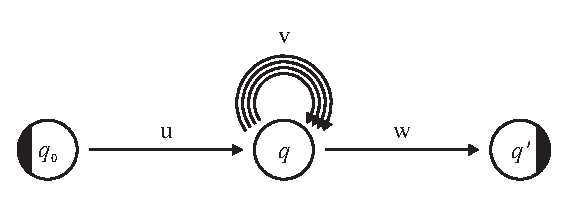
\includegraphics{skript/grafiken/pumping1}
\end{center}

\textbf{Anwendungen:}
\begin{enumerate}
    \item $L = \{ 0^n 1^n \tr n \in \nat \}$ ist \emph{nicht} regul�r. \par
    Angenommen $L$ ist regul�r. Dann gibt es ein $n$ aus dem Pumping-Lemma. \\
    Man nimmt das Wort $z = 0^n 1^n \in L$ mit $|z| \geq n$. \\
    Pumping-Lemma: $z = uvw$, $|uv| \leq n$ und $|v| \geq 1$ \\
    $\Rightarrow$ $u = 0^i$, $v = 0^j$ mit $i + j \leq n$ und $j \geq 1$ \\
    $\Rightarrow$ $uv^2w = 0^{n+j} 1^n \notin L$ \platz Widerspruch! \\
    $\Rightarrow$ $L$ ist \emph{nicht} regul�r.
    \item $L = \{ w \in \{0,1\}^* \tr w^R = w \}$ (Sprache der Palindrome) ist \emph{nicht} regul�r. \par
    Angenommen $L$ ist regul�r. Dann gibt es ein $n$ aus dem Pumping-Lemma. \\
    Man nimmt das Wort $z = 0^n 1 0^n \in L$ mit $|z| \geq n$. \\
    Pumping-Lemma: $z = uvw$, $|uv| \leq n$, $|v| \geq 1$ \\
    $\Rightarrow$ $u = 0^i$, $v = 0^j$ mit $j \geq 1$ \\
    $\Rightarrow$ $uv^2w = 0^{n+j} 1 0^n \notin L$ \platz Widerspruch! \\
    $\Rightarrow$ $L$ ist \emph{nicht} regul�r.
\end{enumerate}

\textbf{Achtung:\;} Nicht in jedem Fall kann man die Nicht-Regularit�t einer Sprache mit dem Pumping-Lemma nachweisen. Das hei�t, es gibt nicht regul�re Sprachen, die das Pumping-Lemma erf�llen. \par \abstand

%%%%%%%%%%%%%%%%%%%%%%%%%%%%%%%%%%%%%%%%%%%%%%%%%%%%%%%%%%%%%%%%%%%%%%%%%%%%%%%
% Zusammenfassung
%%%%%%%%%%%%%%%%%%%%%%%%%%%%%%%%%%%%%%%%%%%%%%%%%%%%%%%%%%%%%%%%%%%%%%%%%%%%%%%
\section{Zusammenfassung}
\begin{eqnarray*}
\text{$L$ ist regul�r} && \left\{ \begin{array}{l}
  \Leftrightarrow \platz \text{$L$ ist DFA-Sprache} \\ \\
  \Leftrightarrow \platz \text{$\Sigma^*_{/ R_L}$ ist endlich} \\ \\
  \Leftrightarrow \platz \text{$\overline{L}$ ist regul�r ($\overline{L} = \{ w \in \Sigma^* \tr w \notin L \}$)} \\ \\
  \Leftrightarrow \platz \text{$L^R$ ist regul�r}
\end{array} \right. \\ \\ \\
\text{$L$ ist regul�r} && \left\{ \begin{array}{l}
  \Rightarrow \platz \text{$L^*$ ist regul�r} \\ \\
  \Rightarrow \platz \text{$L$ erf�llt das Pumping-Lemma}
\end{array} \right. \\ \\ \\
\text{$L_1$ und $L_2$ sind regul�r} && \left\{ \begin{array}{l}
  \Rightarrow \platz \text{$L_1 \circ L_2$ sind regul�r} \\ \\
  \Rightarrow \platz \text{$L_1 \cup L_2$ sind regul�r} \\ \\
  \Rightarrow \platz \text{$L_1 \cap L_2$ sind regul�r}
\end{array} \right.
\end{eqnarray*}

\chapter{Berechenbarkeit}

%%%%%%%%%%%%%%%%%%%%%%%%%%%%%%%%%%%%%%%%%%%%%%%%%%%%%%%%%%%%%%%%%%%%%%%%%%%%%%%
% Turing-Maschinen
%%%%%%%%%%%%%%%%%%%%%%%%%%%%%%%%%%%%%%%%%%%%%%%%%%%%%%%%%%%%%%%%%%%%%%%%%%%%%%%
\section{Turing-Maschinen}
%%%%%%%%%%%%%%%%%%%%%%%%%%%%%%%%%%%%%%%%%%%%%%%%%%%%%%%%%%%%%%%%%%%%%%%%%%%%%%%
\subsection{Einleitung}
\textbf{Idee:\;} Statte einen DFA mit der F�higkeit aus, Informationen zu speichern, zu lesen und zu l�schen. \par \abstand
\begin{center}
    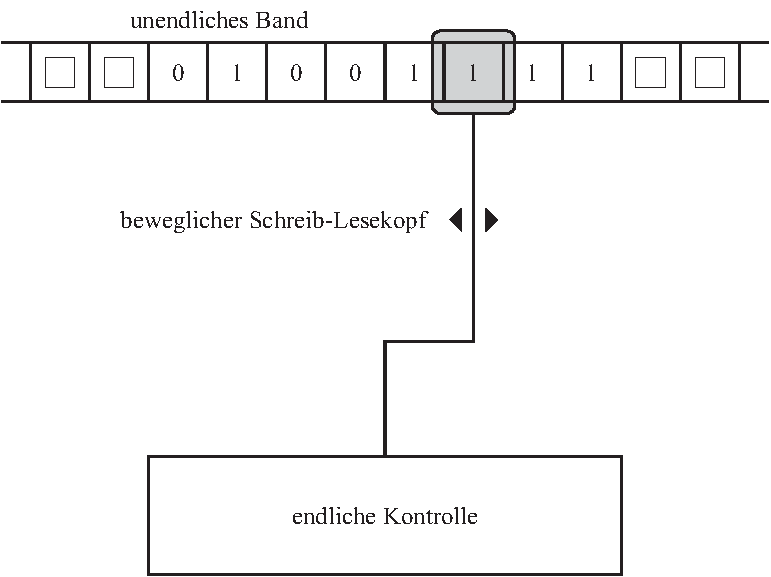
\includegraphics{skript/grafiken/tm}
\end{center}
\pagebreak

\textbf{Definition:\;} Eine \wichtig{Turing-Maschine}\index{TM} (TM) ist gegeben durch ein 7-Tupel.
$$ M=(q, \Sigma, \Gamma, \delta, q_0, \square, F) $$
\begin{itemize}
    \item $Q$: endlicher Zustandsmenge
    \item $\Sigma$: Eingabealphabet
    \item $\Gamma$: Arbeitsalphabet
    \seite
    \item $\delta$: �berf�hrungsfunktion \par
    \begin{center}\begin{tabular}{ccccccccccc}
      $\delta$ & $:$ & $Q$ & $\times$ & $\Gamma$ & $\hookrightarrow$ & $Q$ & $\times$ & $\Gamma$ & $\times$ & $\{L, R, N\}$ \\ \\
               &     & $\uparrow$ &   & $\uparrow$ &             & $\uparrow$ &   & $\uparrow$ &        & $\uparrow$ \\
               &     & { \tiny \begin{tabular}{c} alter \\ Zustand \end{tabular} } & & { \tiny Lesen } &               & { \tiny \begin{tabular}{c} neuer \\ Zustand \end{tabular} } & & \tiny Schreiben& & { \tiny \begin{tabular}{c} Kopf- \\ bewegung \end{tabular} }
    \end{tabular}\end{center}
    \item $q_0$: Anfangszustand
    \item $\square$: Leerzeichen (Blank; $\square \in \Gamma \; \backslash \; \Sigma$)
    \item $F$: Endzust�nde
    \begin{itemize}
        \item Einteitung in akzeptierende und verwerfende m�glich
        \item �berf�hrungsfunktion $\delta$ muss f�r $q \in F$ nicht definiert sein
    \end{itemize}
\end{itemize}
\pagebreak

\textbf{Beispiel:\;} Turing-Maschine f�r $L = \{ 0^n 1^n \tr n \in \nat \}$
\begin{verbatim}
    Solange Band nicht leer
        L�sche eine Null
        Wenn nicht m�glich: Verwerfen
        L�sche eine Eins
        Wenn nicht m�glich: Verwerfen
    Akzeptieren
\end{verbatim}

\begin{center}
    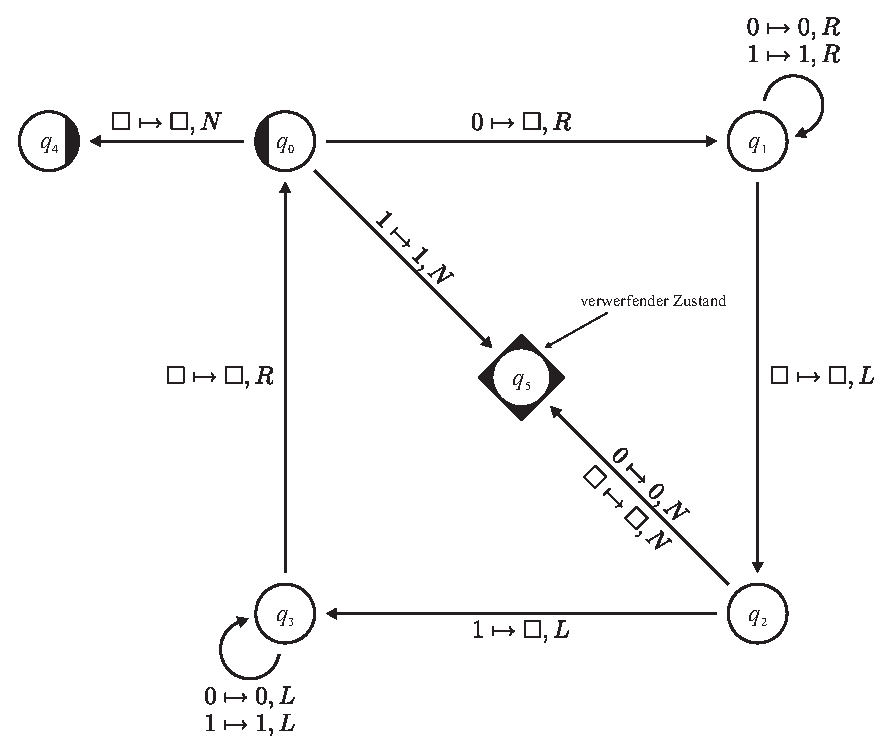
\includegraphics{skript/grafiken/tmnulleneinsen}
\end{center}

\begin{center}\begin{tabular}{r|c|c|c}
        & $0$ & $1$ & $\Box$ \\ \hline
  $q_0$ & $q_1$, $\square$, $R$ & $q_5$, $1$, $N$ & $q_4$, $\square$, $N$ \\
  $q_1$ & $q_1$, $0$, $R$ & $q_1$, $1$, $R$ & $q_2$, $\square$, $L$ \\
  $q_2$ & $q_5$, $0$, $N$ & $q_3$, $\square$, $L$ & ($q_5$, $\square$, $N$) \\
  $q_3$ & $q_3$, $0$, $L$ & $q_3$, 1, $L$ & $q_0$, $\square$, $R$ \\
  akzeptieren $q_4$ & -- & -- & -- \\
  verwerfen $q_5$ & -- & -- & --
\end{tabular}\end{center}
\pagebreak

%%%%%%%%%%%%%%%%%%%%%%%%%%%%%%%%%%%%%%%%%%%%%%%%%%%%%%%%%%%%%%%%%%%%%%%%%%%%%%%
\subsection{Konfiguration}
\textbf{Definition:\;} Eine \wichtig{Konfiguration} ist eine Momentaufnahme der Arbeit einer Turing-Maschine charakterisiert durch Bandinhalt (ohne $\square$), Zustand $q \in Q$ und Kopfposition. \par \abstand
Eine Konfuguration wird repr�sentiert durch $\alpha \; q \; \beta \in \Gamma^* \; Q \; \Gamma^*$.
\begin{itemize}
    \item $\alpha$: Bandinhalt links von Kopfposition
    \item $q$: aktueller Zustand
    \item $\beta$: Bandinhalt ab Kopfposition
\end{itemize}
Die Folgekonfiguration $k'$ einer Konfiguration $k = \alpha \; q \; \beta$ ist bei $\alpha = \alpha' \; a$ und $\beta = b \; \beta'$ folgerma�en charakterisiert:
$$ k' = \left\{ \begin{array}{rcl}
  \alpha' \; q' \; a \; b' \; \beta' & \text{ falls } & \delta(q, b) = (q', b', L) \\ \\
  \alpha \; b' \; q' \; \beta' & \text{ falls } & \delta(q, b) = (q', b', R) \\ \\
  \alpha \; q' \; b' \; \beta' & \text{ falls } & \delta(q, b) = (q', b', N)
\end{array} \right. $$

Schreibweise:
\begin{itemize}
    \item $k \vdash k'$ hei�t $k'$ ist Folgekonfiguration von $k$
    \item $k \overset{*}{\vdash} k'$ hei�t $k = k_0 \vdash k_1 \vdash \ldots \vdash k_m = k'$
\end{itemize}

\textbf{Definition:\;} $\varepsilon \; q_0 \; w$ mit $w \in \Sigma^*$ ist Startkofiguration. \par \abstand

%%%%%%%%%%%%%%%%%%%%%%%%%%%%%%%%%%%%%%%%%%%%%%%%%%%%%%%%%%%%%%%%%%%%%%%%%%%%%%%
\subsection{Berechnung und Entscheidung}
\textbf{Definition:\;} Die \wichtig{Berechnung} einer Turing-Maschine ist eine Konfigurationsfolge
$$k_0 \vdash k_1 \vdash k_2 \vdash k_3 \vdash \ldots$$
die mit der Startkonfiguration beginnt und entweder unendlich ist oder mit einer Endkonfiguration aufh�rt, f�r die keine Folgekonfiguration definiert ist. \par \abstand
Bei einer Endkonfiguration ist der Bandinhalt definiert als Ausgabe. \par \abstand

\textbf{Definition:\;} W�hrend bei einer Berechnung aus einer Eingabe entweder das gesamte Band als Ausgabe folgt (sofern die Turing-Maschine in keine Endlosschleife ger�t), folgt bei der \wichtig{Entscheidung} aus der Eingabe entweder die Ausgabe $0$ (verwerfen) oder $1$ (akzeptieren).
\begin{itemize}
    \item Akzeptierender Endzustand: Band l�schen und $1$ schreiben
    \item Verwerfender Endzustand: Band l�schen und $0$ schreiben
    \item unendliche Berechnungen: Ausgabe nicht definiert
\end{itemize}
\pagebreak

%%%%%%%%%%%%%%%%%%%%%%%%%%%%%%%%%%%%%%%%%%%%%%%%%%%%%%%%%%%%%%%%%%%%%%%%%%%%%%%
\subsection{Codierung endliche Informationsmengen in $Q$}\index{Codierung endliche Informationsmengen in $Q$}\label{codierung}
Durch Erweiterung der Zustandsmenge $Q$ mit einem $k$-stelligen Bitvektor, kann man in jedem Zustand eine fest begrenzte Informationsmenge speichern.
$$ Q' = Q \times \underbrace{ \{ 0, 1 \} \times \{ 0, 1 \} \times \ldots \times \{ 0, 1 \} }_{\text{\tiny $k$ Bit}} $$

\subsection{Erweiterung und Reduktion des Bandalphabets}\index{Erweiterung des Bandalphabets}\index{Reduktion des Bandalphabets}
\textbf{Satz:\;} Das Bandalphabet $\Gamma$ einer Turing-Maschine kann beliebig zu $\Gamma'$ erweitert werden.
$$ \Gamma \platz \Rightarrow \platz \Gamma' \platz \platz \platz (\text{mit } \Gamma \subset \Gamma') $$
\textbf{Satz:\;} Jede Turing-Maschine $M$ mit Bandalphabet $\Gamma$ kann durch eine Turing-Maschine $M'$ mit $\Gamma'~=~\{ 0, 1 \}$ "`simuliert"' werden. \par \abstand
\textbf{Definition:\;} \wichtig{Simulation} ist die Codierung der Konfigurationen von $M$ in Konfigurationen von $M'$.
$$k \platz \mapsto \platz c(k)$$
Jeder Schritt von $M$ wird durch endlich viele Schritte von $M'$ simuliert.
$$ k \vdash k' \platz \mapsto \platz c(k) \vdash c_1 \vdash c_2 \vdash \ldots \vdash c_m \vdash c(k') $$
\textbf{Beweis:}
\begin{itemize}
    \item Codierung von $\Gamma$ in $\{ 0, 1 \}^k$ wobei $k = \left\lceil \log_2 |T| \right\rceil$. Jede Zelle von $M$ wird durch einen Block von $k$ Zellen auf dem Band von $M'$ dargestellt.
    \begin{center}
        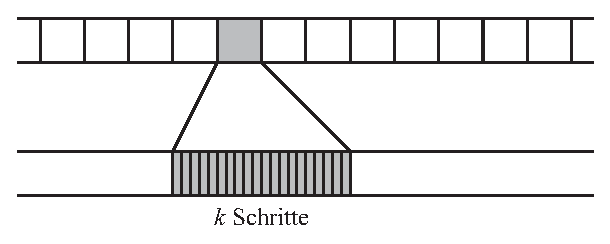
\includegraphics{skript/grafiken/tm1zuk}
    \end{center}
    \pagebreak
    \item Simulation eines Schritts von $M$:
    \begin{itemize}
        \item $M'$ steht auf erster von $k$ Zellen, welche die aktuelle Zelle von $M$ darstellen.
        \item $M'$ geht $k-1$ Schritte nach rechts und "`speichert"' Bandinformation (siehe \ref{codierung}).
        \item $M'$ f�hrt intern �bergangsfunktion von $M$ aus. $M'$ kennt neuen Zustand, Schreibanweisung und Kopfbewegung von $M$.
        \item $M'$ geht $k-1$ Schritte nach links und f�hrt Schreibanweisung aus.
        \item wenn $M$ den Kopf nach links (rechts) bewegt, macht $M'$ $k$ Bewegungen nach nach links (rechts).
    \end{itemize}
    Simulationszeit f�r einen Schritt: $3k - 2$ (konstant)
\end{itemize}

\subsection{Mehrbandmaschinen}\index{Mehrbandmaschinen}
Eine Mehrbandmaschine kann eine endliche Anzahl von B�ndern unabh�ngig voneinander lesen und beschreiben sowie den Schreib-Lesekopf bewegen.
$$\delta : Q \times \Gamma^k \hookrightarrow Q \times \Gamma^k \times \{ L, R, N \}^k$$
\begin{center}
    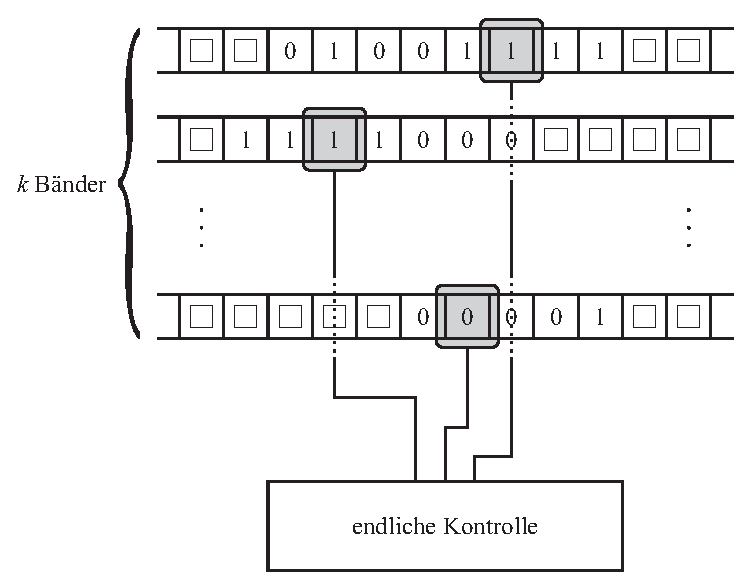
\includegraphics{skript/grafiken/tmmehrband}
\end{center}
\pagebreak
\textbf{Satz:\;} Jede $k$-Band-Turing-Maschine $M$ kann durch eine Ein-Band-Turing-Maschine $M'$ simuliert werden. \par \abstand
\textbf{Beweis:\;} $M'$ simuliert $k$ B�nder durch $k$ Spuren auf einem Band $\Gamma' = \Gamma^k$.
\begin{center}
    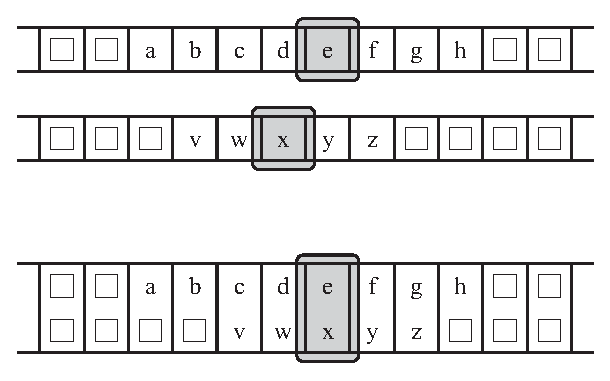
\includegraphics{skript/grafiken/tmmehrbandsimul}
\end{center}
Sofern sich jedoch die K�pfe von $M$ auf den einzelnen B�ndern in unterschiedliche Richtungen bewegen, werden die Spuren $2$ bis $k$ rekonfiguriert, so dass alle Kopfpositionen wieder �bereinander liegen.
\begin{center}
    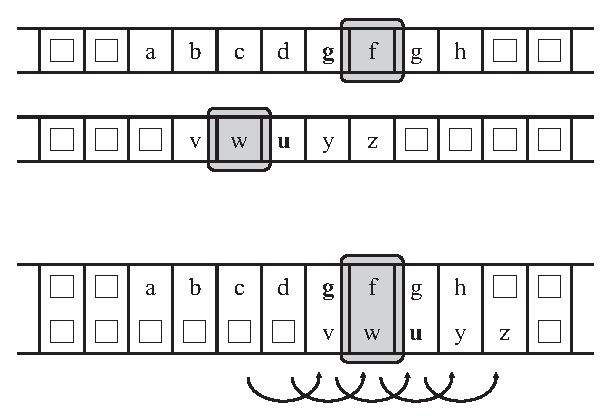
\includegraphics{skript/grafiken/tmmehrbandsimul2}
\end{center}
Simulationszeit: $2 \cdot l$ wobei $l =$ L�nge des beschriebenen Bandes \par \abstand
\textbf{Satz:\;} Jede Berechnung einer $k$-Band-Turing-Maschine $M$ der L�nge $t$ ($t \geq$ Eingabengr��e) kann in $c \cdot t^2$ Zeit ($c$ ist konstant) durch eine Ein-Band-Turing-Maschine simuliert werden.
\pagebreak

\subsection{Verwendung von Unterprogrammen}\index{Unterprogramme}
Die Turing-Maschine $M$ soll ein Unterprogramm (Prozedur) nutzen, das von der Turing-Maschine $M'$ ausgef�hrt wird:
\begin{itemize}
    \item $M$ bekommt zus�tzliches Band und schreibt darauf die �bergabeparameter.
    \item $M'$ rechnet nur auf dem Zusatzband.
    \item $M$ kann Ergebnis auf Zusatzband lesen.
\end{itemize}
Schleifen werden realisiert als Unterprogramme mit Abbruchbedingung.

\subsection{Verkettete Funktionen}\index{Verkettete Funktionen}
Sei $f : \Sigma^* \rightarrow \Gamma^*$ die von $M$ berechnete Funktion. \\
Sei $g : \Gamma^* \rightarrow \Lambda^*$ die von $M'$ berechnete Funktion. \par
Die Maschine $M; M'$ arbeitet wie folgt:
\begin{itemize}
    \item Sie f�hrt alle Schritte so wie $M$ aus.
    \item Falls $M$ stoppt, geht sie auf linkeste beschriebene Stelle des Bandes
    \item $M'$ startet.
\end{itemize}
$M; M'$ berechnet die Funktion $gf : \Sigma^* \rightarrow \Lambda^*$

\subsection{Strukturierung von Ein- und Ausgaben}
Zur Strukturierung von Ein- und Ausgaben wird das Trennsymbol \# verwendet. \par \abstand
\textbf{Beispiel:\;} z.B. $bin(x)\#bin(y)$ als Eingabe f�r Addition
\pagebreak

%%%%%%%%%%%%%%%%%%%%%%%%%%%%%%%%%%%%%%%%%%%%%%%%%%%%%%%%%%%%%%%%%%%%%%%%%%%%%%%
% Church'sche These
%%%%%%%%%%%%%%%%%%%%%%%%%%%%%%%%%%%%%%%%%%%%%%%%%%%%%%%%%%%%%%%%%%%%%%%%%%%%%%%
\section{Church'sche These}\index{Church'sche These}

\textbf{Definition:\;} Eine Relation $f \subseteq A \times B$ beschreibt eine \wichtig{partielle Funktion} von $A$ nach $B$ ($f : A \hookrightarrow B$), wenn jedes $a \in A$ zu h�chstens einem $b \in B$ in Relation steht ($f(a)=b$ falls solch ein $b$ existiert). \par \abstand

\textbf{Definition:\;} Jede Turing-Maschine $M$ berechnet eine partielle Funktion $f_M : \Sigma^* \hookrightarrow \Gamma^*$, wobei $f_M(w)$ nicht definiert ist, wenn $M$ bei Eingabe $w$ nicht h�lt, und der Bandinhalt am Ende der Berechnung $f_M(w)$ ist. Eine Funktion $f_M$ hei�t \wichtig{Turing-berechenbar}. \par \abstand

\textbf{Beobachtung:} ($f : \Sigma^* \hookrightarrow \Gamma^*$)
\begin{center}\begin{tabular}{rcl}
   $f$ ist Turing-berechnenbar & $\Leftrightarrow$ & $f$ ist $\mu$-rekursiv \\
   & $\Leftrightarrow$ & $f$ ist berechenbar mit $\lambda$-Kalk�l \\
   & $\Leftrightarrow$ & $f$ ist berechenbar durch Registermaschinen \\
                     & & (von Neumann-Rechner) \\
   & $\Leftrightarrow$ & $\ldots$
\end{tabular}\end{center}

\textbf{Church'sche These:\;} Die durch die formalen Definitionen der Turing-Bere\-chenbarkeit erfasste Klasse von Funktionen stimmt mit der Klasse der \emph{intuitiv berechnbaren Funktionen}\index{intuitiv berechnbare Funktionen} �berein.
\pagebreak

%%%%%%%%%%%%%%%%%%%%%%%%%%%%%%%%%%%%%%%%%%%%%%%%%%%%%%%%%%%%%%%%%%%%%%%%%%%%%%%
% Primitiv rekursive und �-rekursive Funktionen
%%%%%%%%%%%%%%%%%%%%%%%%%%%%%%%%%%%%%%%%%%%%%%%%%%%%%%%%%%%%%%%%%%%%%%%%%%%%%%%
\section{Primitiv und $\mu$-rekursive Funktionen}
%%%%%%%%%%%%%%%%%%%%%%%%%%%%%%%%%%%%%%%%%%%%%%%%%%%%%%%%%%%%%%%%%%%%%%%%%%%%%%%
\subsection{Einf�hrung}
\textbf{Definition:\;} Die Klasse der \emph{primitiv rekursiven Funktionen}\index{primitiv rekursive Funktion} (kurz: \wichtig{PRF}; $f~:~\nat^k~\rightarrow~\nat$) wird folgerma�en gebildet:
\begin{itemize}
    \item Basisfunktionen:
    \begin{enumerate}
        \item konstante Funktionen ($c, j \in \nat$) \\
        $$ f(x_1, \ldots x_j) = c $$
        \item Projektion ($i, j \in \nat$) \\
        $$ p_{i, j}(x_1, \ldots x_j) = x_i $$
        \item Nachfolgerfunktion \\
        $$ s(x) = x + 1 $$
    \end{enumerate}
    \item Operationen:
    \begin{enumerate}
        \item Funktionskomposition ($j, k \in \nat$ und $g_1, \ldots g_k, h$ sind PRF) \\
        $$ f(x_1, \ldots x_j) = h(g_1(x_1, \ldots x_j), \ldots g_k(x_1, \ldots x_j)) $$ \abstand
        \item Primitive Rekursion ($j \in \nat$ und $g, h$ sind PRF) \\
        \begin{eqnarray*}
            f(0, x_1, \ldots x_j) &=& g(x_1, \ldots x_j) \\
            f(y + 1, x_1, \ldots x_j) &=& h(f(y, x_1, \ldots x_j), y, x_1, \ldots x_j)
        \end{eqnarray*}

    \end{enumerate}
\end{itemize}
\pagebreak

\textbf{Beispiele:}
\begin{enumerate}
    \item Addition
    \begin{eqnarray*}
        \text{\emph{add}} : \nat^2 &\rightarrow& \nat \\
        \text{\emph{add}}(0, x) &=& p_{1, 1}(x) \\
        \text{\emph{add}}(y+1, x) &=& s(p_{1, 3}(\text{\emph{add}}(y, x), y, x)) \\
                                  &=& s(\text{\emph{add}}(y, x))
    \end{eqnarray*}
    \item Multiplikation
    \begin{eqnarray*}
        \text{\emph{mul}} : \nat^2 &\rightarrow& \nat \\
        \text{\emph{mul}}(0, x) &=& 0 \\
        \text{\emph{mul}}(y+1, x) &=& add(p_{1, 3}(\text{\emph{mul}}(y, x), y, x), p_{3, 3}(\text{\emph{mul}}(y, x), y, x)) \\
                                  &=& add(\text{\emph{mul}}(y, x), x)
    \end{eqnarray*}
    \item Vorg�ngerfunktion
    \begin{eqnarray*}
        \text{\emph{pred}} : \nat &\rightarrow& \nat \\
        \text{\emph{pred}}(0) &=& 0 \\
        \text{\emph{pred}}(y+1) &=& p_{2, 2}(\text{\emph{pred}}(y), y)
    \end{eqnarray*}
    \item Pr�dikat ungleich 0
    \begin{eqnarray*}
        \text{\emph{notnull}} : \nat &\rightarrow& \{ 0, 1 \} \\
        \text{\emph{notnull}}(0) &=& 1 \\
        \text{\emph{notnull}}(y+1) &=& 0
    \end{eqnarray*}
    \item Subtraktion (erstes Argument: Minuend, zweites Argument: Subtrahend)
    \begin{eqnarray*}
        \text{\emph{sub}} : \nat^2 &\rightarrow& \nat \\
        \text{\emph{sub}}(0, x) &=& x \\
        \text{\emph{sub}}(y+1, x) &=& pred(p_{1, 3}(\text{\emph{sub}}(y, x), y, x)) \\
                                  &=& pred(\text{\emph{sub}}(y, x)) \\
    \end{eqnarray*}
    \item Pr�dikat kleiner
    \begin{eqnarray*}
        \text{\emph{less}} : \nat^2 &\rightarrow& \{ 0, 1 \} \\
        \text{\emph{less}}(x, y) &=& \text{\emph{notnull}}(\text{\emph{sub}}(x, y))
    \end{eqnarray*}
\end{enumerate}

%%%%%%%%%%%%%%%%%%%%%%%%%%%%%%%%%%%%%%%%%%%%%%%%%%%%%%%%%%%%%%%%%%%%%%%%%%%%%%%
\subsection{$\mu$-Operator}\index{$\mu$-Operator}
Es gibt zwei grunds�tzliche Programmierparadigmen:
\begin{itemize}
    \item Funktionaler Ansatz
    \begin{itemize}
        \item Primitiv rekursive Funktionen
        \item Eigenschaft: total, d.h. �berall definiert
    \end{itemize}
    \item Imperativer Ansatz
    \begin{itemize}
        \item Programm mit elementaren Operationen und \emph{statischen} Schleifen
        \item Eigenschaft: terminiert immer
    \end{itemize}
\end{itemize}
Weder mit primitiv rekursiven Funktionen noch mit imperativen Programmen, die nur statische Schleifen haben, lassen sich alle Turing-berechenbaren Funktion realisieren. Jedoch lassen sich beiden Ans�tze dahingehend erweitern:
\begin{itemize}
    \item Funktionaler Ansatz
    \begin{itemize}
        \item $\mu$-rekursive Funktionen
        \item Eigenschaft: nur partielle Funktionen
    \end{itemize}
    \item Imperativer Ansatz
    \begin{itemize}
        \item Programm mit elementaren Operationen und \verb"while"-Schleifen oder bedingten Sprunganweisungen
        \item Eigenschaft: terminiert \emph{nicht} immer
    \end{itemize}
\end{itemize}

\textbf{Definition:\;} Die $\mu$-Operator ist folgenderma�en definiert:
\begin{eqnarray*}
    g &=& \mu(f) \\
    g(x_1, \ldots x_k) &=& \min\{ n \tr f(n, x_1, \ldots x_k)=0 \text{ und} \\
                       & & \platz \platz \; \text{ $\forall m < n$ ist $f(m, x_1, \ldots x_k)$ definiert} \}
\end{eqnarray*}
Die Klasse der $\mu$-rekursiven Funktionen ist die kleinste Klasse von partiellen Funktionen, die alle primitiv rekursiven Funktionen enth�lt und abgeschlossen ist bez�glich der Anwendung des $\mu$-Operator. \par \abstand

\textbf{Beispiel:\;} Es gibt totale Funktionen, die $\mu$-rekursiv, aber nicht primitiv rekursiv sind, z.B. die Ackermann-Funktion.
\begin{eqnarray*}
    a : \nat^2 &\rightarrow& \nat \\
    a(0, y) &=& y+1 \\
    a(x, 0) &=& a(x-1, 1) \\
    a(x, y) &=& a(x-y, a(x, y-1))
\end{eqnarray*}


%%%%%%%%%%%%%%%%%%%%%%%%%%%%%%%%%%%%%%%%%%%%%%%%%%%%%%%%%%%%%%%%%%%%%%%%%%%%%%%
% Entscheidbarkeit
%%%%%%%%%%%%%%%%%%%%%%%%%%%%%%%%%%%%%%%%%%%%%%%%%%%%%%%%%%%%%%%%%%%%%%%%%%%%%%%
\section{Entscheidbarkeit}\label{entscheidbar}
%%%%%%%%%%%%%%%%%%%%%%%%%%%%%%%%%%%%%%%%%%%%%%%%%%%%%%%%%%%%%%%%%%%%%%%%%%%%%%%
\subsection{Charakteristische Funktion}
\textbf{Definition:\;} Die \wichtig{charakteristische Funktion} $\chi_L : \Sigma^* \rightarrow \{ 0, 1 \}$ und die "`halbe"' charakteristische Funktion $\chi^*_L : \Sigma^* \hookrightarrow \{ 0, 1 \}$ einer Sprache $L \subseteq \Sigma^*$ sind folgenderma�en definiert:
\begin{eqnarray*}
    \chi_L(x) &=& \left\{ \begin{array}{l@{\text{ falls }}l}
    1 & x \in L \\
    0 & x \notin L \end{array} \right. \\ \\
    \chi^*_L(x) &=& \left\{ \begin{array}{l@{\text{ falls }}l}
    1 & x \in L \\
    \text{undefiniert} & x \notin L \end{array} \right.
\end{eqnarray*}

%%%%%%%%%%%%%%%%%%%%%%%%%%%%%%%%%%%%%%%%%%%%%%%%%%%%%%%%%%%%%%%%%%%%%%%%%%%%%%%
\subsection{Entscheidbarkeit und Semi-Entscheidbarkeit}
\textbf{Definitionen:}
\begin{itemize}
    \item Eine Sprache $L$ ist \wichtig{entscheidbar} (rekursiv), wenn die charakteristische Funktion $\chi_L$ Turing-berechenbar ist.
    \item Eine Sprache $L$ ist \wichtig{semi-entscheidbar}, wenn die "`halbe"' charakteristische Funktion $\chi^*_L$ Turing-berechenbar ist.
    \item Eine Sprache $L$ ist \wichtig{rekursiv-aufz�hlbar}, wenn $L$ das Bild einer totalen Turing-berechenbaren Funktion ist.
\end{itemize}

\textbf{Satz:\;} Eine Sprache $L$ ist genau dann entscheidbar, wenn $L$ und $\overline{L} = \Sigma^* \backslash L$ semi-entscheibar sind. \par \abstand
\textbf{Beweis ($\Rightarrow$):\;} Da die Sprache $L$ entscheidbar ist, existiert eine charakteristische Funktion $\chi_L = f_M$ f�r eine Turing-Maschine $M$.
\begin{itemize}
    \item Man konstrutiert zwei Turing-Maschinen $M'$ uns $M''$ f�r $L$ und $\overline{L}$.
    \item $M'$ bzw. $M''$ arbeiten zuerst wie $M$.
    \item Sobald $M$ anh�lt, verhalten sich $M'$ und $M''$ folgenderma�en:
    \begin{itemize}
        \item Falls $M$ akzeptiert, dann akzeptiert auch $M'$ (Symbol $1$ auf das Band schreiben) und $M''$ geht in eine Endlosschleife
        \item Falls $M$ verwirft, dann akzeptiert $M''$ (Symbol $1$ auf das Band schreiben) und $M'$ geht in eine Endlosschleife.
    \end{itemize}
\end{itemize}
Die "`halben"' charakteristischen Funktionen $\chi^*_L$ und $\chi^*_{\overline{L}}$ sind die von den Turing-Maschinen $M'$ und $M''$ berechnete Funktionen:
\begin{eqnarray*}
  \chi^*_L &=& f_{M'} \\
  \chi^*_{\overline{L}} &=& f_{M''}
\end{eqnarray*}
\pagebreak

\textbf{Beweis ($\Leftarrow$):\;} Da die Sprachen $L$ und $\overline{L}$ semi-entscheidbar sind, existieren f�r beide Sprachen die "`halben"' charakteristischen Funktionen $\chi^*_L = f_{M'}$ und $\chi^*_{\overline{L}}~=~f_{M''}$ f�r die Turing-Maschinen $M'$ und $M''$.
\begin{itemize}
    \item Man konstruiert eine 2-Band-Turing-Maschine $M$.
    \item Die Turing-Maschine $M$ kopiert zuerst die Eingabe auf das zweite Band.
    \item Anschliend wird die Maschine $M'$ auf dem ersten Band und $M''$ auf dem zweiten Band simuliert.
    \item Die gesamte Maschine $M$ stoppt, wenn die simulierte Maschine $M'$ oder die simulierte Maschine $M''$ stoppt.
    \item Falls $M'$ gestoppt hat, dann akzeptiert $M$ (Symbol $1$ auf das Band schreiben); falls $M''$ gestoppt hat, dann verwirft $M$ (Symbol $0$ auf das Band schreiben).
\end{itemize}
Die charakteristische Funktion $\chi_L$ ist die von der Turing-Maschine $M$ berechnete Funktion:
$$ \chi_L = f_M $$
\abstand

\textbf{Satz:\;} Die Sprache $L$ ist genau dann rekursiv-aufz�hlbar, wenn $L$ semi-entscheidbar ist. \par \abstand
\textbf{Beweis ($\Rightarrow$):\;} Die Sprache $L$ ist rekursiv-aufz�hlbar. Damit ist $L = \text{Im}(f_M)$, wobei $f_M$ eine totale Funktion ist, die von $M$ berechenbar ist. \par \abstand
Man konstruiert nun eine Maschine $M'$, mit dem Ziel $f_{M'} = \chi^*_L$, denn damit w�re $L$ semi-entscheidbar. \par \abstand
Die Eingabe f�r $M'$ sei $w$ und $M'$ soll akzeptieren, wenn $w \in L$.
\begin{itemize}
    \item Die Maschine $M'$ generiert nacheinander alle Eingaben $u$ f�r $M$ ($u \in \{ \varepsilon, 0, 1, 00, 01, 10, 11, \ldots \} $).
    \item F�r jedes von $M'$ generierte $u$, wird �ber eine Simulation von $M$ der Wert $v = f_M(u)$ berechnet und mit $w$ verglichen:
    \begin{itemize}
        \item Ist $v = w$, dann akzeptiert $M'$ und stoppt.
        \item Ist $v \neq w$, dann wiederholt $M'$ die Berechnung f�r das n�chste $u$.
    \end{itemize}
\end{itemize}
Die "`halbe"' charakteristische Funktion $\chi^*_L$ ist die von der Turing-Maschine $M'$ berechnete Funktion $f_M$, denn die Maschine $M$ h�lt nur, wenn sie eine �bereinstimmung der Eingabe $w$ mit einem Element $v = f_M(u)$ aus dem Bild $\text{Im}(f_M)$ der totalen Funktion $f_M$ findet. Damit ist $L$ semi-entscheidbar.
$$ \chi^*_L = f_{M'} $$

\textbf{Beweis ($\Leftarrow$):\;} Die Sprache $L$ ist semi-entscheidbar. Damit existiert eine "`halbe"' charakteristische Funktion $\chi^*_L = f_{M'}$. \par \abstand
Ziel ist es, eine Maschine $M$ mit der totalen Funktion $f_M$ zu finden, so dass $L = \text{Im}(f_M)$. Die Eingabe f�r $M$ sei $w$.
\begin{itemize}
    \item Man nutzt folgende Bijektion: $\varphi : \nat \rightarrow \nat \times \nat$.
    \begin{center}\begin{tabular}{r|rrrr}
      & 0 & 1 & 2 & 3 \\ \hline
    0 & 0 & 2 & 5 & 9 \\
    1 & 1 & 4 & 8 & 13 \\
    2 & 3 & 7 & 12 & 18 \\
    3 & 6 & 11 & 17 & 24
    \end{tabular}\end{center}
    \item Man setzt voraus, dass $L \neq \emptyset$ und dass Maschine $M$ ein Wort $v \in L$ kennt.
    \item $M$ interpretiet die Eingabe $w \in \Sigma^*$ als $n \in \nat$ und berechnet $\varphi(n) = (n_1, n_2)$.
    \item $M$ interpretiert $bin(n_1)$ ohne die erste $1$ als Eingabe von $M'$ und simuliert $n_2$ Schritte von $M'$. Durch die Begrenzung der Rechenschritte wird verhindert, dass $M'$ in eine Endlosschleife ger�t. Dies ist wichtig, denn die von $M$ berechenbare Funktion muss total sein.
    \item Hat $M'$ das Wort $bin(n_1)$ in $n_2$ Schritten akzeptiert, dann ist $bin(n_1) \in L$, $M$ gibt $bin(n_1)$ aus und stoppt. Sonst gibt $M$ das bekannte Wort $v$ aus und stoppt.
\end{itemize}
Bemerkung: Wenn $bin(n_1)$ in $n_2$ Schritten von $M$ nicht akzeptiert worden ist, hei�t es \emph{nicht}, dass $z = bin(n_1)$ nicht in $L$ ist. F�r ein gr��eres $n$ wiederholt sich aufgrund der Definition von $\varphi$ das Wort $z$ mit einem gr��eren $n_2$, so dass die Zugeh�rigkeit von $z$ zu $L$ mit mehr Schritten �berpr�ft werden kann. \par \abstand
Behauptung: Das Bild der von $M$ berechnete Funktion $f_M$ ist $L$: Ist ein Wort $w \in L$, dann liegt es im Bild von $f_M$ und kann von $M$ nach $n$ Wiederholungen akzeptiert werden, wobei $\varphi(n) = (1w, m)$. Die Maschine $M$ braucht $m$ Schritte, um $w$ zu akzeptieren.
\pagebreak

\textbf{Folgerungen:}
\begin{itemize}
    \item Ist $L$ semi-entscheidbar, aber nicht entscheidbar, dann ist $\overline{L}$ nicht semi-entscheindbar.
    \item $L$ ist genau dann co-semi-entscheidbar, wenn $\overline{L}$ semi-entscheidbar ist.
\end{itemize}
\begin{center}
    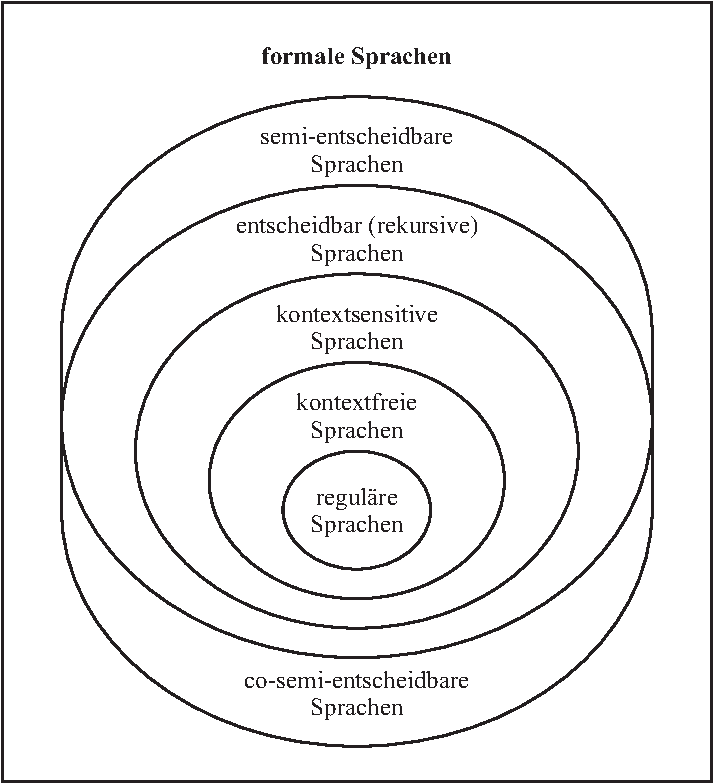
\includegraphics{skript/grafiken/formalesprachen}
\end{center}
\pagebreak

%%%%%%%%%%%%%%%%%%%%%%%%%%%%%%%%%%%%%%%%%%%%%%%%%%%%%%%%%%%%%%%%%%%%%%%%%%%%%%%
% Unentscheidbarkeit
%%%%%%%%%%%%%%%%%%%%%%%%%%%%%%%%%%%%%%%%%%%%%%%%%%%%%%%%%%%%%%%%%%%%%%%%%%%%%%%
\section{Unentscheidbarkeit}
%%%%%%%%%%%%%%%%%%%%%%%%%%%%%%%%%%%%%%%%%%%%%%%%%%%%%%%%%%%%%%%%%%%%%%%%%%%%%%%
\subsection{Einleitung}
Das Ziel ist es zu zeigen, dass es unentscheidbare Sprachen gibt. Das soll mit Hilfe von Diagolanisierung gezeigt werden (wie beim Beweis, dass \emph{keine} Menge $A$ existiert, so dass $|A| = |\pot(A)|$). Dazu wird eine Codierung einer Turing-Maschine als Eingabe f�r eine Turing-Maschine benutzt.

%%%%%%%%%%%%%%%%%%%%%%%%%%%%%%%%%%%%%%%%%%%%%%%%%%%%%%%%%%%%%%%%%%%%%%%%%%%%%%%
\subsection{Codierung von Turing-Maschinen}
Eine Codierung $\langle M \rangle$ f�r eine Turing-Maschine $M$ soll folgenderma�en aussehen:
\begin{itemize}
    \item Alphabet: $\Sigma = \{ 0, 1 \}$ (o.B.d.A.)
    \item Zust�nde: $Q = \{ 1, \ldots n \}$; Startzustand: 1
    \item Arbeitsalphabet: $\Gamma = \{ a_1, \ldots a_m \}$
    \item Zustands�bergangsfunktion: $\delta$ ist eine Folge von $n \cdot m$ Befehlss�tzen:
    $$ \# bin(n) \# bin(m) \# bin(k_1) \# bin(k_2) \# \ldots \# bin(k_{n \cdot m}) $$
    Jedes $k_i$ repr�sentiert eine Zuweisung:
    $$ \delta(p, a_j) = (q, a_k, K) $$
\end{itemize}
\textbf{Satz:\;} Die Sprache $C$ aller g�ltigen Codierungen f�r Turing-Maschinen ist entscheidbar. \label{codierung}
$$ C = \{ w \in \{ 0, 1 \}^* \tr \text{$w$ ist g�ltige Codierung einer TM} \} $$
\textbf{Beweis:\;} Zuerst muss �berpr�ft werden, ob die Codierung $w$ mit zwei Bl�cken beginnt:
$$\# bin(n) \# bin(m) \#$$
Ist dies nicht erf�llt, dann wird das Wort $w$ verworfen. \par \abstand
Ansonsten wird �berpr�ft, ob $m \cdot n$ weitere Bl�cke folgen. Wenn dies nicht der Fall ist, wird $w$ verworfen. \par \abstand
Ansonsten wird jeder einzelne Block auf Korrekkeit gepr�ft. Wenn alle Bl�cke korrekt codiert sind, wird $w$ akzeptiert, sonst wird $w$ verworfen.
\pagebreak

%%%%%%%%%%%%%%%%%%%%%%%%%%%%%%%%%%%%%%%%%%%%%%%%%%%%%%%%%%%%%%%%%%%%%%%%%%%%%%%
\subsection{Universelle Turing-Maschine}
\textbf{Satz:\;} Es gibt eine universelle Turing-Maschine $M_U$, die bei einer Eingabe $\langle M \rangle \# w$ die Arbeit von $M$ auf $w$ simuliert. \par \abstand
\textbf{Beweis:\;} Man konstruiert eine 3-Band-Turing-Maschine:
\begin{itemize}
    \item Band 1: Band von $M$
    \item Band 2: Kopie von $\langle M \rangle$
    \item Band 3: Hilfsband (aktueller Zustand $q$ von $M$)
\end{itemize}
Die Simulation eines Schrittes von $M$ erfolgt folgenderma�en:
\begin{enumerate}
    \item Auf Band $3$ steht der Startzustand von $M$.
    \item $M_U$ liest auf Band $1$ das Symbol $a$ aus $w$.
    \item Anschlie�end sucht $M_U$ den Befehlssatz f�r $\delta(q, a)$ auf Band $2$.
    \item $M_U$ f�hrt die Anweisung auf Band $1$ aus und schreibt den neuen Zustand~$q'$ auf Band $3$.
\end{enumerate}

%%%%%%%%%%%%%%%%%%%%%%%%%%%%%%%%%%%%%%%%%%%%%%%%%%%%%%%%%%%%%%%%%%%%%%%%%%%%%%%
\subsection{Diagonalsprache}
\textbf{Definition:\;} Eine Turing-Maschine bekommt als Eingabe $w$ ihre eigene Codierung. Dieses Wort $w$ soll sie \emph{nicht} akzeptieren. Die Menge aller Codierungen solcher Turing-Maschinen nennt man \wichtig{Diagonalsprache}.
$$ D = \{ w \in \{ 0, 1 \}^* \tr w = \langle M \rangle \text{ und $M$ akzeptiert $w$ \emph{nicht}} \} $$

\textbf{Vorstellung:\;} Es wird in einer Tabelle f�r alle Turing-Maschinen eingetragen, ob sie die Codierung jeder anderen Turing-Maschine oder sich selber akzeptieren oder verwerfen.
\begin{center}\begin{tabular}{c||c|c|c|c|c}
  Eingabe $\backslash$ TMs & $M_1$ & $M_2$ & $M_3$ & $M_4$ & $\cdots$ \\ \hline \hline
  $\langle M_1 \rangle$ & akz. & akz. & verw. & akz. & $\cdots$ \\ \hline
  $\langle M_2 \rangle$ & akz. & \textbf{verw.} & verw. & verw. & $\cdots$ \\ \hline
  $\langle M_3 \rangle$ & verw. & akz. & \textbf{verw.} & akz. & $\cdots$ \\ \hline
  $\langle M_4 \rangle$ & verw. & akz. & akz. & \textbf{verw.} & $\cdots$ \\ \hline
  $\vdots$ & $\vdots$ & $\vdots$ & $\vdots$ & $\vdots$ & $\ddots$
\end{tabular}\end{center}
Nun werden nur die Eintr�ge in der Diagonalen betrachtet, in der jeder Turing-Maschine $M_i$ eine Codierung $\langle M_i \rangle$ zugeordnet wird. Alle Codierungen $\langle M_i \rangle$, bei denen $M_i$ die Codierung $\langle M_i \rangle$ verwirft, geh�ren zur Diagonalsprache $D$. \par \abstand \abstand

\textbf{Satz:\;} Die Diagonalsprache $D$ ist nicht entscheidbar. \par \abstand
\textbf{Beweis (indirekt):\;} Angenommen $D$ sei entscheidbar, dann existiert eine Turing-Maschine $M_D$, so dass die von ihr berechenbare Funktion $f_{M_D}$ die charakteristische Funktion $\chi_D$ ist. \par \abstand
Man benutzt nun die Kodierung $\langle M_D \rangle$ als Eingabe f�r $M_D$:
\begin{itemize}
    \item Angenommen $M_D$ akzeptiert ihre Codierung $\langle M_D \rangle$, dann ist nach der Definition von $D$ ihre Codierung $\langle M_D \rangle \notin D$. Da die von $M_D$ berechnete Funktion $f_{M_D} = \chi_D$ die charakteristische Funktion von $D$ ist, ergibt die Berechnung $\chi_D(\langle M_D \rangle) = 0$, was bedeutet, dass $M_D$ die Codierung $\langle M_D \rangle$ \emph{nicht} akzeptiert. Dies ist ein Widerspruch zur Annahme!
    \item Angenommen $M_D$ akzeptiert ihre Codierung $\langle M_D \rangle$ \emph{nicht}, dann ist nach der Definition von $D$ ihre Codierung $\langle M_D \rangle \in D$. Damit ist $\chi_D(\langle M_D \rangle) = 1$. Also akzeptiert $M_D$ die Codierung $\langle M_D \rangle$. Auch dies ist ein Widerspruch zur Annahme!
\end{itemize}
\begin{center}\begin{tabular}{lcl}
  $M_D$ akzeptiert $\langle M_D \rangle$ & \platz $\Leftrightarrow$ \platz & $\langle M_D \rangle \notin D$ \\
                                         & \platz $\Leftrightarrow$ \platz & $\chi_D(\langle M_D \rangle) = f_{M_D}(\langle M_D \rangle) \neq 1$ \\
                                         & \platz $\Leftrightarrow$ \platz & $M_D$ akzeptiert $\langle M_D \rangle$ nicht \\
                                         &                                 & Widerspruch!
\end{tabular}\end{center}
Daraus folgt: $D$ ist nicht entscheidbar.
\pagebreak

%%%%%%%%%%%%%%%%%%%%%%%%%%%%%%%%%%%%%%%%%%%%%%%%%%%%%%%%%%%%%%%%%%%%%%%%%%%%%%%
\subsection{Spezielles Halteproblem}
\textbf{Definition:\;} Das \emph{spezielle Halteproblem}\index{spezielles Halteproblem}\index{Halteproblem, speziell} (Selbstanwendungsproblem) ist gegeben durch die Sprache \emph{Hs}:
$$ \text{\emph{Hs}} = \{ w \in \{ 0, 1 \}^* \tr \text{$M_w$ angesetzt auf $w$ h�lt} \} $$
Die Turing-Maschine $M_w$ ist definiert als:
$$ M_w = \left\{ \begin{array}{ll}
    M & \text{falls $w = \langle M \rangle$ eine g�ltige Codierung ist}  \\
    \hat{M} & \text{sonst}
  \end{array} \right. $$
Dabei ist $\hat{M}$ eine beliebige, aber fest gew�hlte Turing-Maschine. \par \abstand
\textbf{Satz:\;} Die Sprache \emph{Hs} ist nicht entscheidbar. \par \abstand
\textbf{Beweisidee:\;} Angenommen \emph{Hs} w�re entscheidbar, dann m�sste $D$ auch entscheidbar sein. Dies w�re ein Widerspruch. \par \abstand
\textbf{Beweis (indirekt):\;} Sei $\chi_{\text{\emph{Hs}}}$ die charakteristische Funktion der Sprache \emph{Hs}, dann konstruiert man eine Turing-Maschine $M_D$, so dass die von $M_D$ berechnete Funktion $f_{M_D}$ die charakteristische Funktion $\chi_D$ der Diagonalsprache $D$ ist. Die Eingabe f�r $M_D$ sei $w$.
\begin{enumerate}
    \item $M_D$ entscheidet, ob $w = \langle M \rangle$ eine g�ltige Codierung ist (siehe \ref{codierung}).
    \begin{itemize}
        \item Wenn ja: $M_D$ f�hrt fort
        \item Wenn nein: $M_D$ verwirft
    \end{itemize}
    \item $M_D$ nutzt $M_{\text{\emph{Hs}}}$ und entscheidet, ob $M = M_w$ auf $w$ h�lt
    \begin{itemize}
        \item Wenn ja: $M_D$ f�hrt fort
        \item Wenn nein: $M_D$ akzeptiert, da die Maschine $M$ sich damit nicht akzeptieren kann und deswegen zu $D$ geh�rt.
    \end{itemize}
    \item $M_D$ nutzt die Universal-Turing-Maschine $T_U$, um die Berechnung von $M = M_w$ bei Eingabe $w$ zu simulieren (es ist nun bekannt, dass $M_w$ bei Eingabe $w$ terminiert).
    \begin{itemize}
        \item Wenn $M_w$ die Eingabe $w$ akzeptiert, verwirft $M_D$ die Eingabe.
        \item Wenn $M_w$ die Eingabe $w$ verwirft, akzeptiert $M_D$ die Eingabe.
    \end{itemize}
\end{enumerate}
Damit existiert eine charakteristische Funktion $\chi_D = f_{M_D}$. Daraus folgt, dass die Diagonalsprache $D$ entscheidbar ist. Dies ist ein Widerspruch! \par \abstand
Daraus folgt: \emph{Hs} ist \emph{nicht} entscheidbar.

\pagebreak

%%%%%%%%%%%%%%%%%%%%%%%%%%%%%%%%%%%%%%%%%%%%%%%%%%%%%%%%%%%%%%%%%%%%%%%%%%%%%%%
% Reduktion
%%%%%%%%%%%%%%%%%%%%%%%%%%%%%%%%%%%%%%%%%%%%%%%%%%%%%%%%%%%%%%%%%%%%%%%%%%%%%%%
\section{Reduktionen}
%%%%%%%%%%%%%%%%%%%%%%%%%%%%%%%%%%%%%%%%%%%%%%%%%%%%%%%%%%%%%%%%%%%%%%%%%%%%%%%
\subsection{Definition der Reduktion}\index{Reduktion}
\textbf{Definition:\;} Es seien $L_1 \subseteq \Sigma_1^*$ und $L_2 \subseteq \Sigma_2^*$ Sprachen. \par \abstand
$L_1$ ist reduzierbar auf $L_2$, wenn eine totale berechenbare Funktion $f : \Sigma_1^* \rightarrow \Sigma_2^*$ existiert, so dass f�r alle $w \in \Sigma_1^*$ gilt:
$$ w \in L_1 \platz \Leftrightarrow \platz f(w) \in L_2 $$
Schreibweise:
$$ L_1 \leq L_2 $$ \abstand

\textbf{Lemma:\;} Ist $L_1 \leq L_2$ und ist $L_2$ entscheidbar (bzw. semi-entscheidbar), dann ist auch $L_1$ entscheidbar (bzw. semi-entscheidbar). \par \abstand
\textbf{Beweis:\;} Sei $L_1 \leq L_2$ mittels $f$ und $L_2$ sei entscheidbar. Daraus folgt, dass die charakteristische Funktion $\chi_{L_2}$ berechenbar ist. Zu zeigen ist Berechenbarkeit der charakterischen Funktion $\chi_{L_1}$. \par \abstand
Um zu entscheiden, ob ein Wort $w$ in der Sprache $L_1$ liegt, wird $f(w)$ berechnet und entschieden, ob $f(w)$ in $L_2$ liegt. Wenn dies Fall ist, ist auch $w \in L_1$; wenn nicht, dann ist $w \notin L_2$.
\begin{eqnarray*}
    \chi_{L_1} &=& \chi_{L_2} \circ f \\ \\
    \chi_{L_1}(w) = 1 & \Leftrightarrow & w \in L_1 \\
                      & \Leftrightarrow & f(w) \in L_2 \\
                      & \Leftrightarrow & \chi_{L_2}(f(w)) = 1
\end{eqnarray*}
Damit ist $\chi_{L_1}$ berechenbar. Daraus folgt, dass $L_1$ entscheidbar ist. \par \abstand
F�r den Beweis f�r semi-entscheidbare Sprachen ist $\chi_{L_1}$ durch $\chi^*_{L_1}$ und $\chi_{L_2}$ durch $\chi^*_{L_1}$ zu ersetzen.
\pagebreak

%%%%%%%%%%%%%%%%%%%%%%%%%%%%%%%%%%%%%%%%%%%%%%%%%%%%%%%%%%%%%%%%%%%%%%%%%%%%%%%
\subsection{Allgemeines Halteproblem}
\textbf{Definition:\;} Das \emph{allgemeine Halteproblem}\index{allgemeine Halteproblem}\index{Halteproblem, allgemein} ist gegeben durch die Sprache $H$:
$$ H = \{ w\#x \tr \text{$M_w$ angesetzt auf $x$ h�lt} \} $$
Die Turing-Maschine $M_w$ ist definiert als:
$$ M_w = \left\{ \begin{array}{ll}
    M & \text{falls $w = \langle M \rangle$ eine g�ltige Codierung ist}  \\
    \hat{M} & \text{sonst}
  \end{array} \right. $$
\textbf{Satz:\;} Die Sprache $H$ ist nicht entscheidbar. \par \abstand
\textbf{Beweis:\;} Es ist zu zeigen, dass $\text{\emph{Hs}} \leq H$. W�re $H$ entscheidbar, m�sste \emph{Hs} auch entscheidbar sein. Dies w�re ein Widerspruch. \par \abstand
Gesucht wird eine Funktion $f$ f�r die Reduktion, so dass $w \in \text{\emph{Hs}} \Leftrightarrow f(w) \in H$. Es wird folgede Zuweisung gew�hlt:
$$ f(w) = w\#w $$
Probe:
$$ w \in \text{\emph{Hs}} \platz \Leftrightarrow \platz \text{$M_w$ h�lt auf $w$} \platz \Leftrightarrow \platz w\#w \in H $$
Damit ist \emph{Hs} auf $H$ reduzierbar. Da aber \emph{Hs} nicht entscheidbar ist, ist auch $H$ nicht entscheidbar.

%%%%%%%%%%%%%%%%%%%%%%%%%%%%%%%%%%%%%%%%%%%%%%%%%%%%%%%%%%%%%%%%%%%%%%%%%%%%%%%
\subsection{Halteproblem auf leerem Band}
\textbf{Definition:\;} Das \wichtig{Halteproblem auf leerem Band} ist gegeben durch die Sprache~$H_0$:
$$ H_0 = \{ w \tr \text{$M_w$ angesetzt auf $\varepsilon$ h�lt} \} $$
\textbf{Satz:\;} Die Sprache $H_0$ ist nicht entscheidbar. \par \abstand
\textbf{Beweis:\;} Es ist zu zeigen, dass $H \leq H_0$. W�re $H_0$ entscheidbar, m�sste $H$ auch entscheidbar sein. Dies w�re ein Widerspruch. \par \abstand
Es wird folgende Funktion f�r die Reduktion gew�hlt: Man ordnet jedem Wort $w\#x$ eine Turing-Maschine zu, die bei Start auf leerem Band $x$ auf das Band schreibt und sich dann wie $M_w$ verh�lt. Man bezeichnet mit $f(w\#x)$ die Codierung dieser Maschine.
\begin{eqnarray*}
    w\#x \in H &\Leftrightarrow& \text{$M_w$ h�lt auf $x$} \\
               &\Leftrightarrow& \text{die durch $f(w\#x)$ beschriebene Maschine h�lt auf leerem Band} \\
               &\Leftrightarrow& f(w\#x) \in H_0
\end{eqnarray*}
Damit ist $H$ auf $H_0$ reduzierbar. Da aber $H$ nicht entscheidbar ist, ist auch $H_0$ nicht entscheidbar.
\pagebreak

%%%%%%%%%%%%%%%%%%%%%%%%%%%%%%%%%%%%%%%%%%%%%%%%%%%%%%%%%%%%%%%%%%%%%%%%%%%%%%%
\subsection{Universalsprache}
\textbf{Definition:\;} Die Universalsprache $U$ ist folgenderma�en definiert:
$$ U = \{ w\#x \tr \text{$M_w$ angesetzt auf $x$ akzeptiert} \} $$
Die Turing-Maschine $M_w$ ist folgenderma�en definiert, wobei hier $\hat{M}$ eine Turing-Maschine ist, die immer akzeptiert:
$$ M_w = \left\{ \begin{array}{ll}
    M & \text{falls $w = \langle M \rangle$ eine g�ltige Codierung ist}  \\
    \hat{M} & \text{sonst}
  \end{array} \right. $$
\textbf{Satz:\;} Die Sprache $U$ ist nicht entscheidbar. \par \abstand
\textbf{Beweis:\;} Es ist zu zeigen, dass $\overline{D} \leq U$ und $\overline{D}$ nicht entscheidbar ist. \par \abstand
Die Sprache $\overline{D}$ ist nicht entscheidbar, da $D$ nicht entscheidbar ist.
$$ \overline{D} = \{ w \in \{ 0, 1 \}^* \tr \text{$w \neq \langle M \rangle$ oder ($w = \langle M \rangle$ und $M$ akzeptiert $w$)} \} $$
Es wird folgende Funktion f�r die Reduktion gew�hlt:
$$ f(w) = w\#w $$
Probe:
\begin{eqnarray*}
    w \in \overline{D} &\Leftrightarrow& \text{$w \neq \langle M \rangle$ oder ($w = \langle M \rangle$ und $M$ akzeptiert $w$)} \\
                       &\Leftrightarrow& \text{$M_w = \hat{M}$ oder $M_w = M$ und $M_w$ akzeptiert $w$} \\
                       &\Leftrightarrow& \text{$M_w$ akzeptiert $w$ (da $\hat{M}$ alles akzeptiert)} \\
                       &\Leftrightarrow& w\#w \in U
\end{eqnarray*}
Damit ist $\overline{D}$ auf $U$ reduzierbar. Da aber $\overline{D}$ nicht entscheidbar ist, ist auch $U$ nicht entscheidbar. \par \abstand \abstand
\pagebreak

\textbf{Satz:\;} Die Universalsprache $U$ ist semi-entscheidbar. \par \abstand
\textbf{Beweis:\;} Es existiert eine Turingmaschine $M$, so dass die von $M$ berechnete Funktion $f_{M}$ die "`halbe"' charakteristische Funktion $\chi^*_U$ der Universalsprache $U$ ist:
\begin{enumerate}
    \item Die Maschine $M$ �berpr�ft zuerst, ob die Eingabe die Form $w\#x$ hat
    \begin{itemize}
        \item Wenn ja: $M$ f�hrt fort
        \item Wenn nein: $M$ geht in eine Endlosschleife
    \end{itemize}
    \item $M$ simuliert $M_w$ mit der Eingabe $x$
    \item Falls $M_w$ h�lt, wird gepr�ft, ob $M_w$ das Wort $x$ akzeptiert hat
    \begin{itemize}
        \item Wenn ja: $M$ akzeptiert die Eingabe $w\#x$
        \item Wenn nein: $M$ geht in eine Endlosschleife
    \end{itemize}
    \item Hinweis: Sollte $M_w$ nicht halten, kann $M$ auch nicht halten.
\end{enumerate}
\abstand

\textbf{Satz:\;} Die Sprache $\overline{U}$ ist \emph{nicht} semi-entscheidbar. \par \abstand
\textbf{Beweis (indirekt):\;} Angenommen $\overline{U}$ ist semi-entscheidbar. Da $U$ semi-entscheidbar ist, w�rde aus der Semi-Entscheidbarkeit von $U$ und $\overline{U}$ folgen, dass $U$ entscheidbar ist. Dies w�re ein Widerspruch.
\pagebreak

%%%%%%%%%%%%%%%%%%%%%%%%%%%%%%%%%%%%%%%%%%%%%%%%%%%%%%%%%%%%%%%%%%%%%%%%%%%%%%%
\subsection{Postsches Korrespondenzproblem}
\textbf{Definition:\;} Das \emph{Postsche Korrespodenzproblem}\index{Postsches Korrespodenzproblem} ist gegeben durch die Sprache~\emph{PCP}\index{PCP}:
$$ \text{\emph{PCP}} = \{ (u_1, v_1), \ldots (u_k, v_k) \tr \exists i_1 \ldots i_n \platz u_{i_1} \circ \ldots \circ u_{i_n} = v_{i_1} \circ \ldots \circ v_{i_n} \} $$
\begin{eqnarray*}
    & \vdots & \\
    & \vdots & \\
    & \vdots & \\
    & \text{Vorlesung vom 12.6.2002 (fehlt)} & \\
    & \vdots & \\
    & \vdots & \\
    & \vdots &
\end{eqnarray*}

\chapter{Komplexit�t}

%%%%%%%%%%%%%%%%%%%%%%%%%%%%%%%%%%%%%%%%%%%%%%%%%%%%%%%%%%%%%%%%%%%%%%%%%%%%%%%
% Die Komplexit�tsklasse P
%%%%%%%%%%%%%%%%%%%%%%%%%%%%%%%%%%%%%%%%%%%%%%%%%%%%%%%%%%%%%%%%%%%%%%%%%%%%%%%
\section{Die Komplexit�tsklasse $\bigP$}
%%%%%%%%%%%%%%%%%%%%%%%%%%%%%%%%%%%%%%%%%%%%%%%%%%%%%%%%%%%%%%%%%%%%%%%%%%%%%%%
\subsection{Komplexit�tsklassen}
\textbf{Definition:\;} Ist $M$ eine Turing-Maschine und $w \in \Sigma^*$, dann bezeichnet $\stime_M(w)$ die Anzahl der Schritte die $M$ bei der Eingabe $w$ macht:
$$ \stime_M : \Sigma^* \rightarrow \nat \cup \{ \infty \} $$
\textbf{Definition:\;} Sei $f : \nat \rightarrow \nat$ eine Funktion. Die \wichtig{Komplexit�tsklasse} $\btime(f(n))$ besteht aus allen Sprachen $L$, f�r die eine Mehrband-Turing-Maschine $M$ existiert, mit der Eigenschaft $L = L(M)$ und die Anzahl der Schritte $\stime_M(w)$, die $M$ bei der Eingabe $w$ macht, ist kleiner oder gleich $f(|w|)$ f�r alle $w \in \Sigma^*$. Insbesondere gilt, dass $M$ immer h�lt.
\begin{eqnarray*}
    \btime(f(n)) &=& \{ L \subseteq \Sigma^* \tr \text{$\exists$ TM $M$ mit $L(M) = L$ und } \\
                 & & \text{ $\forall w \in \Sigma^* \; \stime_M(w) \leq f(|w|)$} \}
\end{eqnarray*}

\textbf{Beispiel:\;} Die Nachfolgerfunktion $s : \nat \rightarrow \nat$ ist folgenderma�en definiert:
$$ s(n) = n + 1 $$
Alle regul�ren Sprachen $L_{\text{regul�r}}$ liegen in der Komplexit�tsklasse $\btime(s(n))$. \par \abstand \abstand

%%%%%%%%%%%%%%%%%%%%%%%%%%%%%%%%%%%%%%%%%%%%%%%%%%%%%%%%%%%%%%%%%%%%%%%%%%%%%%%
\subsection{Polynomialzeitprobleme}
\textbf{Definition:\;} Die Komplexit�tsklasse $\bigP$ der "`Polynomialzeitprobleme"' ist folgenderma�en definiert:
\begin{eqnarray*}
    \bigP &=& \{ L \tr \text{$\exists$ TM $M$ \; $\exists$ Polynom $p(n)$} \\
          & & \text{ mit $L = L(M)$ und $\forall w \in \Sigma^* \; \stime_M(w) \leq p(|w|)$} \} \\ \\
    \bigP &=& \bigcup_{p(n) \text{ Poylnom}} \btime(p(n)) \\ \\
    L \in \bigP &\Leftrightarrow& \text{$\exists$ TM $M$ \; $\exists k \in \nat$ \; $\forall w \in \Sigma^*$ \; $L = L(M)$ \; $\stime_M(w) = \bigO(|w|^k)$}
\end{eqnarray*}
Die Klasse $\bigP$ stimmt mit der Klasse der in Polynomialzeit entscheidbaren Probleme auf Registermaschinen �berein, wenn alle Operationen mit logarithmischem Kostenma� angerechnet werden (d.h. Kosten f�r eine Zuweisung, Addition etc. sind gleich der Anzahl der beteiligten Bits). \par \abstand

\textbf{Erweiterte Church'sche These:\;} Die Klasse $\bigP$ ist die Klasse der effizient berechenbaren Probleme. \par \abstand

\textbf{Konsequenz:\;} Zum Nachweis, dass $L \in \bigP$, reicht es aus, die Algorithmen (Pseudocode, Flussdiagramme etc.) zu analysieren. \par \abstand

\textbf{Beispiele:\;} Folgende Sprachen liegen in $\bigP$:
\begin{itemize}
    \item $\{ p(x)\#n \tr \text{$p(x)$ ist rationales Polynom, $n \in \nat$ und $p(n) = 0$} \}$ \par
    Begr�ndung: Horner-Schema
    \item $\{ \langle \text{lineares Gleichungssystem} \rangle \tr \text{das System hat eine L�sung} \}$ \par
    Begr�ndung: Gauss-Elimination
    \item $\{ bin(a)\#bin(b)\#bin(c) \tr \text{$a, b, c, \in \nat$ und $ggT(a, b) = c$} \}$ \par
    Begr�ndung: Euklidischer Algorithmus
    \item $\{ \langle G \rangle \tr \text{Graph $G$ ist zusammenh�ngend} \}$ \par
    Begr�ndung: Tiefensuche (DFS) bzw. Breitensuche (BFS)
\end{itemize}

\textbf{Beispiele:\;} Von folgenden Problemen ist nicht bekannt, ob sie in $\bigP$ liegen (wahrscheinlich nicht):
\begin{itemize}
    \item $\text{\emph{HAM}} = \{ \langle G \rangle \tr \text{$G$ hat einen Hamilton-Kreis} \}$ \par
    Bemerkung: Ein Hamilton-Kreis ist ein Kreis, der jeden Knoten genau einmal besucht.
    \item $\text{\emph{PRIME}} = \{ bin(n) \tr \text{$n$ ist eine Primzahl} \}$
\end{itemize}
\pagebreak

%%%%%%%%%%%%%%%%%%%%%%%%%%%%%%%%%%%%%%%%%%%%%%%%%%%%%%%%%%%%%%%%%%%%%%%%%%%%%%%
% Die Komplexit�tsklasse NP
%%%%%%%%%%%%%%%%%%%%%%%%%%%%%%%%%%%%%%%%%%%%%%%%%%%%%%%%%%%%%%%%%%%%%%%%%%%%%%%
\section{Die Komplexit�tsklasse $\bigNP$}
%%%%%%%%%%%%%%%%%%%%%%%%%%%%%%%%%%%%%%%%%%%%%%%%%%%%%%%%%%%%%%%%%%%%%%%%%%%%%%%
\subsection{Nichtdeterministische Turing-Maschinen}
\textbf{Hinweis:\;} Die bisherige Definition von Turing-Maschinen war deterministisch. Das hei�t, jede Konfiguration hat eine eindeutige (oder keine) Nachfolgekonfiguration. \par \abstand

\textbf{Definition:\;} Eine \wichtig{nichtdeterministische Turing-Maschine}\index{Turing-Maschine, nichtdeterministisch} (kurz: \wichtig{NTM}) ist ein 7-Tupel:
$$ M = (Q, \Sigma, \Gamma, \delta, q_0, \Box, F) $$
Alle Komponenten bis auf $\delta$ sind wie bei der deterministischer Turing-Maschine.
\begin{itemize}
    \item $\delta$: Zustands�berf�hrungsfunktion
    $$ \delta : Q \times \Gamma \rightarrow \pot(Q \times \Gamma \times \{ L, R, N \}) $$
    Falls $\delta(q, a) = \emptyset$, stoppt die Turing-Maschine. \par
    Endkonfigurationen sind immer akzeptierend oder verwerfend.
\end{itemize}

\textbf{Definition:\;} Eine nichtdeterministische Turing-Maschine $M$ akzeptiert eine Eingabe $w$ genau dann, wenn im Baum der Folgekonfigurationen mindestens ein Weg von der Startkonfiguration $\varepsilon q_0 w$ zu einer akzeptierenden Endkonfiguration f�hrt. Die akzeptierenden W�rter bilden die Sprache $L(M)$. \par \abstand
\begin{center}
    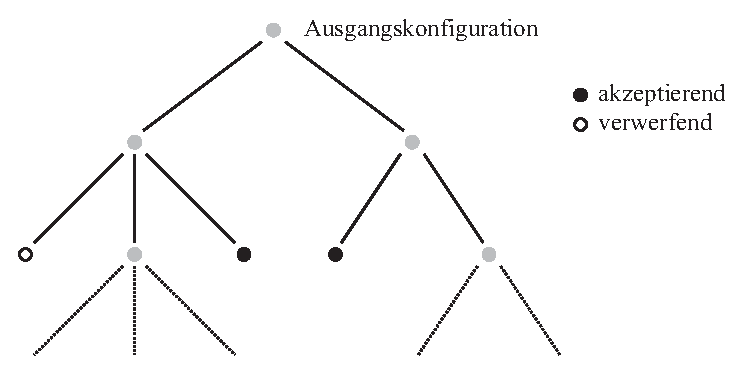
\includegraphics{skript/grafiken/ntm}
\end{center}
\pagebreak

%%%%%%%%%%%%%%%%%%%%%%%%%%%%%%%%%%%%%%%%%%%%%%%%%%%%%%%%%%%%%%%%%%%%%%%%%%%%%%%
\subsection{Komplexit�tsklassen}
\textbf{Definition:\;} F�r jede nichtdeterministische Turing-Maschine $M$ existiert die Funktion $\sntime_M$:
$$ \sntime_M(w) = \left\{ \begin{array}{ccl}
  \begin{array}{l}
    \text{Minimale Wegl�nge von $\varepsilon q_0 w$} \\
    \text{zu einer akzeptierenden Endkonfiguration}
  \end{array} & \text{ falls } & w \in L(M) \\ \\
  0 & \text{ falls } & w \notin L(M)
\end{array} \right. $$

\textbf{Definition:\;} Sei $f : \nat \rightarrow \nat$ eine Funktion. Die Komplexit�tsklasse $\bntime(f(n))$ besteht aus allen Sprachen $L$, f�r die eine nichtdeterministische Mehrband-Turing-Maschine $M$ existiert, mit der Eigenschaft $L = L(M)$ und die minimale Anzahl der Schritte $\sntime_M(w)$ von der Startkonfiguration $\varepsilon q_0 w$ zu einer akzeptierenden Endkonfiguration, ist kleiner oder gleich $f(|w|)$ f�r alle $w \in \Sigma^*$.
\begin{eqnarray*}
    \bntime(f(n)) &=& \{ L \subseteq \Sigma^* \tr \text{$\exists$ NTM $M$ mit $L(M) = L$} \\
                  & & \text{ und $\forall w \in \Sigma^* \; \sntime_M(w) \leq f(|w|)$} \}
\end{eqnarray*}

%%%%%%%%%%%%%%%%%%%%%%%%%%%%%%%%%%%%%%%%%%%%%%%%%%%%%%%%%%%%%%%%%%%%%%%%%%%%%%%
\subsection{Effizient verifizierbare Probleme}
\textbf{Definition:\;} Die Komplexit�tsklasse $\bigNP$ der effizient (in Polynomialzeit) verfizierbaren Probleme ist folgenderma�en definiert:
$$ \bigNP = \bigcup_{p(n) \text{ Poylnome}} \bntime(p(n)) $$
\begin{center}
    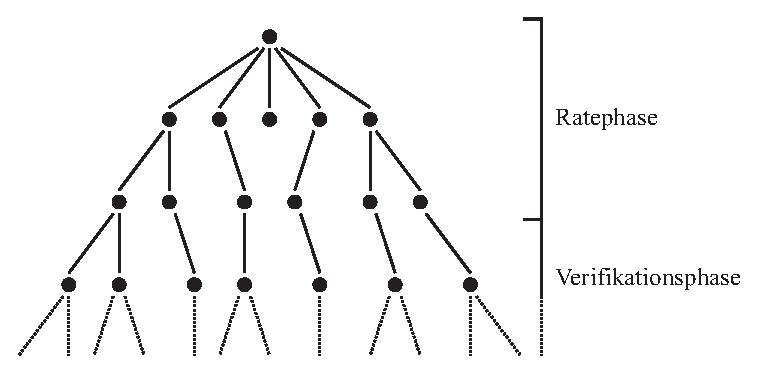
\includegraphics{skript/grafiken/ratenverifizieren}
\end{center}
\pagebreak

\textbf{Beispiele:\;} Folgende Sprachen liegen in $\bigNP$:
\begin{itemize}
    \item Alle Sprachen $L \in \bigP$ \par
    Begr�ndung: $\bigP \subseteq \bigNP$
    \item $\text{\emph{COMPOSITE}} = \{ bin(n) \tr \text{$n > 1$ und $n$ ist keine Primzahl} \}$ \par
    Bemerkung: Test auf zusammengesetzte Zahlen \par
    \begin{itemize}
        \item $M$ r�t $bin(k)$ und $bin(l)$ wobei $1 < |bin(k)|, |bin(l)| \leq |bin(n)|$.
        \item $M$ pr�ft, ob $k \cdot l = n$ ($bin(n)$ ist Eingabe) in $c \cdot |bin(n)|^2$ Zeit.
        \begin{itemize}
            \item[--] Wenn ja: $M$ akzeptiert
            \item[--] Wenn nein: $M$ geht in eine Endlosschleife
        \end{itemize}
    \end{itemize}
    \item $\text{\emph{HAM}} = \{ \langle G \rangle \tr \text{$G$ hat einen Hamilton-Kreis} \}$ \par
    \begin{itemize}
        \item $M$ r�t eine Permutation der Knoten von $G$.
        \item $M$ pr�ft, ob die Permutation einen Kreis in $G$ beschreibt.
        \begin{itemize}
            \item[--] Wenn ja: $M$ akzeptiert
            \item[--] Wenn nein: $M$ geht in eine Endlosschleife
        \end{itemize}
    \end{itemize}
\end{itemize}
Bemerkung:\; Das Raten erfolgt bitweise, d.h. die Maschine schreibt eine zuf�llige Anzahl zuf�lliger Bits auf ein Band und �berpr�ft dann beispielsweise, ob die geratene Bitfolge eine Permutation repr�sentiert.
\pagebreak

%%%%%%%%%%%%%%%%%%%%%%%%%%%%%%%%%%%%%%%%%%%%%%%%%%%%%%%%%%%%%%%%%%%%%%%%%%%%%%%
% NP-Vollst�ndigkeit
%%%%%%%%%%%%%%%%%%%%%%%%%%%%%%%%%%%%%%%%%%%%%%%%%%%%%%%%%%%%%%%%%%%%%%%%%%%%%%%
\section{$\bigNP$-Vollst�ndigkeit}
%%%%%%%%%%%%%%%%%%%%%%%%%%%%%%%%%%%%%%%%%%%%%%%%%%%%%%%%%%%%%%%%%%%%%%%%%%%%%%%
\subsection{Polynomiale Reduktion}
\textbf{Definition:\;} Eine Sprache $L_1 \subseteq \Sigma^*$ ist auf $L_2 \subseteq \Gamma^*$ polynomial reduzierbar, falls eine totale von einer Polynomialzeit-beschr�nkten deterministischen Turing-Maschine berechenbare Funktion $f : \Sigma^* \rightarrow \Gamma^*$ existiert, so dass
$$ w \in L_1 \platz \Leftrightarrow \platz f(w) \in L_2 $$
Schreibweise:
$$L_1 \leq_{\bigP} L_2$$
\abstand

\textbf{Satz:\;} Ist $L_1 \leq_{\bigP} L_2$ und $L_2 \in \bigP$, dann ist $L_1 \in \bigP$. \par \abstand
\textbf{Beweis:\;} Es sei $w \in \Sigma^*$ und $|w| = n$.
\begin{itemize}
    \item Bestimme $f(w)$ in $p(n)$ Schritten
    $$ \Rightarrow |f(w)| \leq p(n) $$
    \item Pr�fe, ob $f(w) \in L_2$ in $q(p(n))$ Zeit.
    $$ \Rightarrow \text{Polynomialzeit} $$
    $f(w) \in L_2 \platz \Leftrightarrow \platz w \in L_1$
\end{itemize}
\textbf{Folgerung:\;} Ist $L_1 \leq L_2$ und $L_1 \notin \bigP$, dann ist $L_2 \notin \bigP$.

%%%%%%%%%%%%%%%%%%%%%%%%%%%%%%%%%%%%%%%%%%%%%%%%%%%%%%%%%%%%%%%%%%%%%%%%%%%%%%%
\subsection{$\bigNP$-vollst�ndige Probleme}
\textbf{Definition:\;} Eine Sprache $L$ ist $\bigNP$-schwer (auch: $\bigNP$-hart), falls f�r alle $L' \in \bigNP$ gilt, dass $L' \leq_{\bigP} L$. \par \abstand
\textbf{Definition:\;} $L$ ist $\bigNP$-vollst�ndig, falls $L$ $\bigNP$-schwer und $L \in \bigNP$. \par \abstand
\pagebreak

%%%%%%%%%%%%%%%%%%%%%%%%%%%%%%%%%%%%%%%%%%%%%%%%%%%%%%%%%%%%%%%%%%%%%%%%%%%%%%%
\subsection{\emph{SAT}-Erf�llbarkeitsproblem}
\textbf{Definition:\;} Das \wichtig{Erf�llbarkeitsproblem f�r Formeln der Aussagenlogik} ist gegeben durch die Sprache \emph{SAT}\index{SAT} ($F$ ist eine Codierung einer Formel):
$$ \text{\emph{SAT}} = \{ \langle F \rangle \in \Gamma^* \tr \text{$F$ ist erf�llbar} \} $$

\textbf{Satz:\;} Die Sprache \emph{SAT} liegt in $\bigNP$. \par \abstand

\textbf{Beispiel:}
$$ F = (x_1 \lor x_2) \land (\neg x_1 \lor x_2) \land (\neg x_1 \lor x_2) $$
Hinweis:\; $F$ ist erf�llbar durch $x_1 = 0$ und $x_2 = 1$. \par \abstand
Vorgehen:
\begin{itemize}
    \item $M$ r�t eine Belegung der Variablen in $F$.
    \item $M$ berechnet den Wert von $F$ unter dieser Belegung.
    \begin{itemize}
        \item Wenn der Wert 1 ist: $M$ akzeptiert
        \item Wenn der Wert 0 ist: $M$ geht in eine Endlosschleife
    \end{itemize}
\end{itemize}
\abstand

\textbf{Satz (Cook / Levin):\;} Das Erf�llbarkeitsproblem f�r Formeln der Aussagenlogik \emph{SAT} ist $\bigNP$-vollst�ndig. \par \abstand
\textbf{Beweis:}
\begin{enumerate}
    \item Es ist zu zeigen, dass \emph{SAT} $\bigNP$-schwer ist, d.h. f�r beliebiges $L \in \bigNP$ gilt $L \leq_{\bigP} \text{\emph{SAT}}$, d.h. es gilt eine totale in Polynomialzeit berechenbare Funktion $f : \Sigma^* \rightarrow \Gamma^*$, so dass $w \in L \platz \Leftrightarrow \platz f(w) \in \text{\emph{SAT}}$.
    \item Idee: $L \in \nat \bigP$, d.h. $\exists \; \text{NTM } M$
    \begin{itemize}
        \item $L = L(M)$
        \item $M$ ist Polynomialzeit-beschr�nkt
        $$ w = a_1, a_2, \ldots a_n \platz \text{Eingabe f�r $M$} $$
        $$ w \in L \platz \Leftrightarrow \platz \text{$M$ erreicht einen akzeptiereden Endzustand bei Eingabe $w$} $$
        Codiere Berechnung von $M$ auf $w$ durch Formel, die genau dann erf�llbar ist, wenn $M$ akzeptierende Endkofiguration erreichen kann. \par \abstand
        Vereinfachung: $Q = \{ q_0, q_1 \ldots q_k \}$ \par \abstand
        $M$ akzeptiert durch einen akzeptierenden Endzustand $q_{\text{\tiny accept}} \in Q$ (nicht mit $1$ auf Band).
    \end{itemize}
\end{enumerate}
\pagebreak

\begin{eqnarray*}
    & \vdots & \\
    & \vdots & \\
    & \vdots & \\
    & \text{Vorlesung vom 21.6.2002 (fehlt)} & \\
    & \vdots & \\
    & \vdots & \\
    & \vdots &
\end{eqnarray*}

\chapter{Kontextfreie Sprachen}

%%%%%%%%%%%%%%%%%%%%%%%%%%%%%%%%%%%%%%%%%%%%%%%%%%%%%%%%%%%%%%%%%%%%%%%%%%%%%%%
% Grammatiken und die Chomsky-Hierarchie
%%%%%%%%%%%%%%%%%%%%%%%%%%%%%%%%%%%%%%%%%%%%%%%%%%%%%%%%%%%%%%%%%%%%%%%%%%%%%%%
\section{Grammatiken und die Chomsky-Hierarchie}

\textbf{Hinweis:\;} Eine \emph{Grammatik} ist ein System, um Ausdr�cke (W�rter) nach bestimmten Regeln zu bilden, und beschreibt eine Sprache. \par \abstand
\textbf{Bemerkung:\;} Dieses Prinzip ist bereits aus der Bildung von Formeln, Termersetzungsverfahren, Aufbau von Programmiersprachen bekannt. \par \abstand
\textbf{Definition:\;} Eine Grammatik ist eine 4-Tupel $G = (V, \Sigma, P, S)$:
\begin{itemize}
    \item $V$: endliche Menge von Variablen (Gro�buchstaben)
    \item $\Sigma$: endliches Terminalalphabet ($\Sigma \cap V = \emptyset$)
    \item $S \in V$: Startvariable
    \item $P$: endliche Menge von Regeln (Produktionen)
    $$ P \subseteq (\Sigma \cup V)^+ \times (\Sigma \cup V)^* $$
\end{itemize}

Ist $u = xyz, v = xy'z \in (\Sigma \cup V)^*$ und ist $(y, y') \in P$, dann sagen wir, dass $v$ aus $u$ ableitbar (unter G) ist (oder $u$ geht in $v$ �ber). Wir schreiben daf�r:
$$ u \Longrightarrow_G v \platz (\text{kurz: } u \Longrightarrow v \platz) $$

$\overset{*}{\Longrightarrow}_G$ ist reflexiver und transitiver Abschluss von $\Longrightarrow_G$, d.h. $u \overset{*}{\Longrightarrow}_G v$, wenn $u = u_0 \Longrightarrow_G u_1 \Longrightarrow_G \ldots \Longrightarrow_G u_k = v $
$$ L(G) = \{w \in \Sigma^* \tr S \overset{*}{\Longrightarrow}_G w \} $$
\pagebreak

\textbf{Beispiel:}
\begin{enumerate}
    \item Korrekte Klammerausdr�cke:
    $$ G = ( \{ S \}, \{ (, ) \}, P, S ) \platz \text{mit} \platz P = \{ (S, ()), (S, (S)), (S, SS) \} $$
    Ableitung und Syntaxbaum:
    \begin{eqnarray*}
        S &\Longrightarrow_G& S\underline{S} \\
          &\Longrightarrow_G& S(\underline{S}) \\
          &\Longrightarrow_G& \underline{S}(SS) \\
          &\Longrightarrow_G& ()(S\underline{S}) \\
          &\Longrightarrow_G& ()(\underline{S}()) \\
          &\Longrightarrow_G& ()(()())
    \end{eqnarray*}
    \item Palindrome
    $$ G = ( \{ S \}, \{ 0, 1 \}, P, S ) \platz \text{mit} \platz P = \{ (S, 0), (S, 1), (S, 00), (S, 11), (S, 0S0), (S, 1S1) \} $$
    Beispiel:
    $$ 10001: S \Longrightarrow 1S1 \Longrightarrow 10S01 \Longrightarrow 10001 $$
    K�rzere Darstellung der Regeln mit einer Variable auf der linken Seite:
    $$ S \rightarrow 0 \tr 1 \tr 00 \tr 11 \tr 0S0 \tr 1S1 $$
    Nennt man \wichtig{Backus-Naur-Form} (\wichtig{BNF})
\end{enumerate}

\textbf{Definition:}
\begin{itemize}
    \item Jede Grammatik ist (zun�chst) vom Typ 0 (keine Einschr�nkung).
    \item Eine Grammatik ist vom Typ 1 (kontextsensitiv), falls f�r alle Regeln $w_1 \rightarrow w_2$ gilt: $|w_1| \leq |w_2|$.
    \item Eine Grammatik ist vom Typ 2 (kontextfrei), falls f�r alle Regeln $w_1 \rightarrow w_2$ so sind, dass $w_1 \in V$ und $|w_2| \geq 1$
    \item Eine Grammatik ist vom Typ 3 (regul�r), falls f�r alle Regeln $w_1 \rightarrow w_2$ so sind, dass $w_1 \in V$ und $w_2 \in \Sigma \cup \Sigma V$
\end{itemize}
\pagebreak

%%%%%%%%%%%%%%%%%%%%%%%%%%%%%%%%%%%%%%%%%%%%%%%%%%%%%%%%%%%%%%%%%%%%%%%%%%%%%%%
\section{Kontextfreie Sprachen und Normalform}
\textbf{Definition:\;} Sprache $L$ ist kontextfrei, wenn eine Typ 2-Grammatik existiert, so dass $L = L(G)$. \par \abstand
\textbf{Beispiel:\;} $L = \{ a^n b^n \tr n \in \natpos \}$ ist kontextfrei (aber nicht regul�r).
$$ S \rightarrow ab \tr aSb $$

\textbf{Definition:\;} Eine kontextfreie Grammatik $G$ mit $\varepsilon \notin L(G)$ ist in \wichtig{Chomsky-Normalform} (kurz: \wichtig{CNF}), falls alle Regeln die folgende Form haben:
\begin{eqnarray*}
    A \rightarrow a & & A \in V, a \in \Sigma \\
    A \rightarrow BC & & A, B, C \in V
\end{eqnarray*}

CNF impliziert bin�re Syntaxb�ume der Ableitungen, wenn man den letzten Schritt der Umwandlung in Terminalsymbole vernachl�ssigt. \par \abstand
\textbf{Beispiel:\;} CNF von $L = \{ a^n b^n \tr n \in \natpos \}$:
\begin{eqnarray*}
    S &\rightarrow& AT \\
    T &\rightarrow& SB \tr b \\
    A &\rightarrow& a \\
    B &\rightarrow& b
\end{eqnarray*}
\begin{center}
    GRAFIK: Bin�rbaum f�r $aabb$
\end{center}

Schematisch:
\begin{center}
    GRAFIK: Dreick (bin�r) mit Rechteck drunter (letzter Schritt)
\end{center}

\textbf{Satz:\;} F�r jede kontextfreie Grammatik $G$ existiert eine CNF $G'$, so dass $L(G) = L(G')$ (d.h. $G$ und $G'$ sind �quivalent). \par \abstand
\textbf{Beweis:}
\begin{enumerate}
    \item Elemination von Regeln der Form $A \rightarrow B$
    \begin{enumerate}
        \willbuch
        \item Wenn ein Kreis $A_1 \rightarrow A_2 \rightarrow \ldots \rightarrow A_k \rightarrow A_1$ ersetze $A_1, A_2, \ldots A_k$ durch neue Variable $A$ (f�r alle Regeln).
        \item wenn weiterhin eine Regel $B_1 \rightarrow B_2$ existiert, streichen diese Regel und erg�nzen die aus $B_1$ abgeleiteten Regeln mit denen, die aus $B_2$ abgeleitet werden.
    \end{enumerate}
    \item Alle Regeln haben die Form
    $$ A \rightarrow a \platz \text{oder} \platz A \rightarrow x \in (V \cup \Sigma)^* $$
    \begin{enumerate}
        \willbuch
        \item F�r jedes $a \in \Sigma$ f�gt man ein neues $B_a$ zu $V$ hinzu sowie die Regeln $B_a \rightarrow a$.
        \item Regel $A \rightarrow x = A_1 A_2 b_1 A_3 b_2$ wird ersetzt durch (am Beispiel)
        $$ A \rightarrow A_1 A_2 B_{b_1} A_3 B_{b_2} $$
        \item F�r jeden Suffix der L�nge $\geq 2$ Hilfsvariable einf�hren (am Beispiel)
        \begin{eqnarray*}
            A \rightarrow A_1 C_1 \\
            C_1 \rightarrow A_2 C_2 \\
            C_2 \rightarrow B_{b_1} C_3 \\
            C_3 \rightarrow A_3 B_{b_2}
        \end{eqnarray*}
    \end{enumerate}
\end{enumerate}

\textbf{Anwendung:\;} Umformung f�r $S \rightarrow ab \tr aSb$:
\begin{eqnarray*}
    A &\rightarrow& a \\
    B &\rightarrow& b \\
    S &\rightarrow& AB \tr AC \\
    C &\rightarrow& SB
\end{eqnarray*}

\textbf{Definition:\;} Eine kontextfreie Grammatik ist in \wichtig{Greibach Normalform} (kurz: \wichtig{GNF}), falls alle Regeln die Form $A \rightarrow a B_1 \ldots B_k$ ($k \in \nat$) haben. \par \abstand
\textbf{Satz:\;} F�r jede kontextfreie Grammatik gibt es eine �quivalente GNF (ohne Beweis). \par \abstand

\textbf{CYK-Algorithmus:}
\begin{itemize}
    \item Gegeben: $G = (V, \Sigma, P, S)$ in CNF und $w = a_1, a_2, \ldots a_n \in \Sigma^*$
    \item Frage: $w \in L(G)$ ?
    \item Idee: $w \in L(G)$ betrachte oberste Stufe des Syntaxbaums einer Ableitung: $S \Longrightarrow_G AB$, dann wird aus $A$ ein Pr�fix von $w$ abgeleitet, aus $B$ ein Suffix.
    \item Cocke, Younger, Kasami: Anwendung von dynamischer Programmierung
    $$ w_{i, j} = \underbrace{a_i a_{i+1} \ldots a_{i+j-1}}_{\text{f�ngt mit $a_i$ an und hat L�nge $j$}} $$
    $$ T_{i, j} = \{ A \in V \tr A \overset{*}{\Rightarrow}_G w_{i, j} \} $$
    $$ S \in T_{1, n} \platz \Leftrightarrow \platz S \overset{*}{\Rightarrow}_G w_{1, n} \platz \Leftrightarrow \platz w \in L(G) $$
    \item Initialisierung:
    $$ T_{i, 1} = \{ A \tr (A, a_i) \in P \} $$
    \begin{itemize}
        \item[] \verb"for i = 2 to n"
        \begin{itemize}
            \item[] \verb"for i = 1 to n - j + 1"
            $$ T_{i, j} = \bigcup_{k = 1}^{j - 1} \{ A \tr \exists B \in T_{i, k}, C \in T_{i + k, j - k} \text{ und } (A, B C) \in P \} $$
        \end{itemize}
    \end{itemize}
    \item Laufzeit: $\bigO(n^3)$
\end{itemize}

%%%%%%%%%%%%%%%%%%%%%%%%%%%%%%%%%%%%%%%%%%%%%%%%%%%%%%%%%%%%%%%%%%%%%%%%%%%%%%%
\section{Pumping-Lemma}
\textbf{Satz:\;} F�r jede kontextfreie Sprache $L$ existiert ein $n \in \nat$, so dass f�r jedes $z \in L$ mit $|z| \geq n$ eine Zerlegung $z = uvwxy$ existiert mit:
\begin{itemize}
    \item $|vwx| \leq n$
    \item $|vx| \geq 1$
    \item $\forall i \in \nat$ ist $z' = u v^i w x^i y \in L$
\end{itemize}

\textbf{Beispiele:}
\begin{enumerate}
    \item $L = \{ a^k b^k \tr k \in \nat \}$ ist kontextfrei, also erf�llt es das Pumping-Lemma. \par \abstand
    Man setzt $n = 2$ imd betrachtet ein $z \in L$ mit $|z| \geq n = 2$. Dann ist
    $$ z = a^k b^k \text{ mit } k \geq 1 $$
    und man findet eine Zerlegung
    $$ z = \underbrace{a \ldots}_{u} \underbrace{a}_{v} \underbrace{\varepsilon}_{w} \underbrace{b}_{x} \underbrace{\ldots b}_{y} $$
    Wie man leicht sieht:
    $$ z' = uv^i w x^i y = a^{k+(i-1)} b^{k+(i-1)} \in L $$
    \item $L = \{ a^k b^k c^k \tr k \in \nat \}$ ist nicht kontextfrei. \\
    Indirekter Beweis: Angenommen $L$ w�re kontextfrei, dann gibt es ein $n$ aus dem Pumping-Lemma, $\ldots$ \\
    \begin{eqnarray*}
        a^n b^n c^n &=& uvwxy \\
        \text{Aus 1) } vwx &\in& \underbrace{a^* b^*}_{\text{Fall 1}} \cup \underbrace{b^* c^*}_{\text{Fall 2}} \\
        z' = u v^2 w x^2 y
    \end{eqnarray*}
    \begin{itemize}
        \item Fall 1: Anzahl der $a$'s oder Anzahl der $b$'s in $z'$ ist $>n$, Anzahl der $c$'s gleich $n$ \\
        $\Rightarrow z' \notin L \Rightarrow$ Widerspruch
        \item Fall 2: Anzahl der $b$'s oder Anzahl der $c$'s in $z'$ ist $>n$, Anzahl der $a$'s gleich $n$ \\
        $\Rightarrow z' \notin L \Rightarrow$ Widesrspruch
    \end{itemize}
    Widerspruch zur Annahme, d.h. $L$ ist nicht kontextfrei.
\end{enumerate}

\textbf{Beweis der Pumping-Lemmas:\;} Sei $G$ CNF f�r $L$.
$$ G = (V, \Sigma, P, S) $$
Man definiert: $k = |V|$ und $n := 2^k$ \\
Sei $z \in L$ mit $|z| \geq n$ \\
Aufgabe: Zerlegung finden \\
Syntaxbaum $T$ f�r eine Ableitung von $z$ ohne Terminalsymbole ist bin�r und hat $|z|$ Bl�tter. Daraus folgt, dass die Tiefe von $T \geq k$. \\
Man betrachtet einen Weg maximaler L�nge (also $\geq k$), dann muss auf dem Weg eine Variable doppelt austreten. \\
Man betrachtet erste Variablendopplung von unten und die entsprechenden Unterb�ume
\begin{center}
    GRAFIK: Unterb�ume
\end{center}
Beide haben h�chstens Tiefe $k$ h�chstens $2^k = n$ Bl�tter. \\
Zerlegung $uvwxy$:
\begin{itemize}
    \item $|vwx| \leq n$, da gr��erer Baum $\leq n$ Bl�tter hat
    \item $|vx| \geq 1$, da die B�ume verschieden sind (kleiner Baum ist Unterbaum)
    \item $z' = u v^j w x^j y = uwy$ wird durch folgenden baum abgebildet:
    \begin{center}
        GRAFIK: kleinen Baum nach oben
    \end{center}
    $z'' = u v^2 w x^2 y$
    \begin{center}
        GRAFIK: gro�er Baum doppelt
    \end{center}
    Jede weitere $u v^{i+1} w x^{i+1} y$ durch Ersetzung des kleinen Baum durch den gro�en
\end{itemize}

%%%%%%%%%%%%%%%%%%%%%%%%%%%%%%%%%%%%%%%%%%%%%%%%%%%%%%%%%%%%%%%%%%%%%%%%%%%%%%%
\section{Kellerautomaten}
\textbf{Idee:\;} Automat darf Eingabe nur einmal von links nach rechts lesen und kann Informationen in einem Kellerspeicher aufbewahren.
\begin{center}
    GRAFIK: Schema
\end{center}
Formel:\; Ein nichtdeterministischer Kellerautomat (kurz: \wichtig{NPDA}) wird durch ein 6-Tupel beschrieben:
$$ M = (Q, \Sigma, \Gamma, \delta, q_0, \#) $$
\begin{itemize}
    \item $Q$: endliche Zustandsmenge
    \item $\Sigma$: Eingabealphabet (kleine Buchstaben)
    \item $\Gamma$: Kelleralphabet (gro�e Buchstaben)
    \item $\delta$: Zustands�berf�hrungsfunktion
    $$ \delta : Q \times (\Sigma \cup \{ \varepsilon \}) \times \Gamma \rightarrow \underset{e}{\pot}(Q \times \Gamma^*) $$
    $\underset{e}{\pot}$ hei�t: Menge aller endlichen Teilmengen
    \item $q_0 \in Q$: Startzustand
    \item $\# \in \Gamma$: unterstes Kellerzeichen
\end{itemize}

\textbf{Arbeitsweise:\;} $(q', B_1 \ldots B_k) \in \delta(q, a, A)$ \\
Wenn $M$ im Zustand $q$ und $a$ auf dem Band und $A$ in oberster Kellerzelle liest, so kann er in $q'$ �bergehen, $A$ l�schen und $B_1 \ldots B_k$ in den Keller speichern ($B_1$ oben). \\
$(q', B_1 \ldots B_k) \in \delta(q, \varepsilon, A)$ \\
Wenn $M$ im Zustand $q$ auf oberster Kellerzelle $A$ liest, kann er ohne Eingabesymbol zu lesen in $q'$ �bergehen, $A$ l�schen und $B_1 \ldots B_k$ speichern. \\

\textbf{Konfiguration:\;} $k \in \underbrace{Q}_{\text{aktueller Zustand}} \times \underbrace{\Sigma^*}_{\text{ungelesen}} \times \underbrace{\Gamma^*}_{\text{Kellerinhalt}}$ \\
$k \vdash k'$: $k'$ ist direkte Folgekonfiguration von $k$ \\
$k \overset{*}{\vdash} k'$: $k = k_0 \vdash k_1 \vdash \ldots \vdash k_n = k'$ \\

\textbf{Akzeptierende Endkonfiguration:\;} $(q, \varepsilon, \varepsilon)$ wobei $q$ beliebig \\

\textbf{Definition:\;} $w \in L(M) \platz \Leftrightarrow \platz (q_0, w, \#) \overset{*}{\vdash} (q, \varepsilon, \varepsilon)$


% Indexverzeichnis
\printindex

\end{document}
